\documentclass[12pt,a4paper]{report}
\usepackage[a4paper, top=0.98in, bottom=0.98in, left=1.85in, right=0.79in]{geometry}
\usepackage{graphicx}
\usepackage{fancyhdr}  % For custom headers and footers
\usepackage{titlesec}  % For customizing title formats
\usepackage{setspace}  % For line spacing
\usepackage[absolute,overlay]{textpos}
\usepackage{tikz}
\usetikzlibrary{positioning}
\usepackage{booktabs} % For better-looking tables
\usepackage{amsmath} 
\usepackage{url}
\usepackage{xcolor} % for text coloring
\usepackage{listings}
\usepackage{amsmath}
\usepackage{subcaption}



% Format chapter titles
\titleformat{\chapter}[display]
{\normalfont\Huge\bfseries}{\chaptertitlename\ \thechapter}{20pt}{\Huge}
\titlespacing*{\chapter}{0pt}{0pt}{18pt} % Set the first number to 0pt for top spacing


% Set up spacing
\onehalfspacing




% let it number up to subsubsection
\setcounter{secnumdepth}{3}

% Make sure chapter titles appear correctly in the header
\renewcommand{\chaptermark}[1]{\markboth{#1}{}}

\begin{document}

% Cover page
\newcommand{\titlefont}{\fontfamily{ptm}\fontsize{18}{22}\selectfont\bfseries}

\begin{titlepage}
    
    \begin{tikzpicture}[overlay, remember picture]
        % Vertical line
        \draw[thick] (current page.south west) ++(1.7in, 0) -- ++(0, \paperheight - 2.1in); 
        
    \end{tikzpicture}

   \begin{textblock*}{1cm}(1.0in, 5in)  % Adjust position as needed
   	\centering
   	\rotatebox{-90}{
   		\begin{minipage}{14cm}  % Adjust width as needed
   			\centering
   			Mosaned | Navigation and Guidance System for Indoor Environments for Blind and Visually Impaired Individuals 
   		\end{minipage}
   	}
   \end{textblock*}
   
    \vspace*{1.2in}
    \centering
    
     % Uni coordinates for the image placement
    \begin{textblock*}{1.04in}(0.7in,3.3in)
    
\includegraphics[width=0.576in,height=0.7488in]{assets/uni.png}
    \end{textblock*}
    
    % Uni coordinates for the image placement
    \begin{textblock*}{1.04in}(2.2in,1in)
    
\includegraphics[width=0.8in,height=1.04in]{assets/uni.png}
    \end{textblock*}

    % Dep. coordinates for the image placement
    \begin{textblock*}{1.04in}(6in,1.1in)
    
\includegraphics[width=1.4in,height=1.04in]{assets/dep.png}
    \end{textblock*}

    {\titlefont \textbf{Taibah University}}\\
    {\titlefont \textbf{College of Computer Science Engineering}}\\
    {\titlefont \textbf{Computer Engineering Department}}\\
    
    \vspace{1.8cm}
    
    {\titlefont \textbf{Mosaned | Navigation and Guidance System for Indoor Environments for Blind and Visually Impaired Individuals}}
    
    \vspace{1.8cm}

    {\titlefont \fontsize{14}{16} \textbf{A Project Submitted in partial fulfilment of the requirements for the Bachelor Degree in Computer Engineering}}
    \vspace{1.8cm}
    
    \vspace{1.2cm}
    
    \begin{minipage}{\textwidth}
    	\centering
    	{\titlefont \textbf{Submitted By}}\\
    	\vspace{1cm}
    	
    	\begin{tabular}{@{}l@{\hskip 4cm}r@{}}
    		{\titlefont \textbf{Mohammed Alharbi}} & {\titlefont \textbf{4200174}} \\
    		{\titlefont \textbf{Firas Alsadeq}} & {\titlefont \textbf{4200625}} \\
    		{\titlefont \textbf{Mousa Alenzi}} & {\titlefont \textbf{4106574}} \\
    	\end{tabular}
    \end{minipage}
    
    \vspace{1.8cm}

    {\fontfamily{ptm}\selectfont\fontsize{14}{16}\normalfont
    \textbf{Project Advisor}\\
    Dr. Moteb Alghamdi
    }
    
    \vspace{2cm}

    {\fontfamily{ptm}\selectfont\fontsize{14}{16}\normalfont
    \textless 2024-2025\textgreater-\textless 1st Semester\textgreater
    }

\end{titlepage}


\pagenumbering{roman}



\newpage
\thispagestyle{plain}
\setcounter{page}{1}
\renewcommand{\thepage}{\roman{page}}

\begin{center}
    \Large\textbf{ABSTRACT}
\end{center}
\vspace{6pt}


Visually impaired and blind individuals might face difficult challenges when navigating through indoor environments, especially if they where not familiar with them. Indoor environments can be very unpredictable and filled with obstacles, and they are rich of important visual information which only designed for eyes consumption. These difficulties rise the need of these individuals to assistants and guiders whether by asking strangers, or by taking companions. But
these solutions will lead to decreasing the independence of these individuals. We are trying to offer a solution in this project, a wearable and easy to use system that guides and assists the users after determining their positions and scanning their surrounding environments using only a camera and smart phone. The proposed system is an integration of three systems: Objects Detection, Localization, and Customizable Guidance System. These components rely on analyzing the images captured by a camera and extracting the important visual information from them. The Objects Detection System can detects the surrounding objects and describe them to the users if they asked to, and informusers about obstacles, and users can ask it to alarm them when they face an object with certain characteristics, such as a main wearing red T-Shirt. The localization system will use the camera to detect artificial landmarks to determine the user’s location. And finally, the Customizable Guidance System reads to user custom information and instructions after entering specific areas. \\
\textcolor{red} {
	- the result obtained\\
	- the significance of the result or finding 
}





\vspace{18pt}
\noindent
\textbf{KEYWORDS:}  Localization; Obstacles Avoidance; Objects Detection, Customization; Guidance; Pose; Calibration
\vspace{3\baselineskip}
\newpage
\thispagestyle{plain}
\setcounter{page}{2}
\renewcommand{\thepage}{\roman{page}}

\begin{center}
    \Large\textbf{ACKNOWLEDGEMENTS}
\end{center}
\vspace{6pt}

The content of this single page is left to the preference of the student.  It is suggested however that the page makes reference to guidance received by the student from his or her supervisor and project Committee members.  Reference should also be made to any financial assistance received to carry out the project.  Any extraordinary assistance received by the student for example in word processing, data collection, data analysis, and so on, should be properly acknowledged.  The acknowledgements should not exceed 250 words.
\color{black}

% Table of Contents
\clearpage
\vspace{0pt} % Remove any vertical spacing
\tableofcontents




\clearpage
\addcontentsline{toc}{chapter}{List of Tables}
\listoftables
\color{black}


\clearpage
\addcontentsline{toc}{chapter}{List of Figures}
\listoffigures
\color{black}


\clearpage
\color{red}

\chapter*{Glossary and List of Abbreviations}

\section*{Glossary}
\begin{description}
  \item[Term 1] Definition of term 1.
  \item[Term 2] Definition of term 2.
\end{description}

\section*{List of Abbreviations}
\begin{description}
  \item[Abbr.] Full form of the abbreviation.
\end{description}

\color{black} % Include glossary and list of abbreviations
\addcontentsline{toc}{chapter}{Glossary and List of Abbreviations} 


% Reset page numbering and start Arabic numbering

\clearpage
\pagenumbering{arabic}
\setcounter{page}{1} % Start Arabic page numbering from 1

% Set up fancyhdr for custom headers
\pagestyle{fancy}
\fancyhf{} % Clear all header and footer fields
\fancyhead[L]{\text{Chapter \thechapter{}} - \small{\leftmark}}

\fancyfoot[C]{\thepage} % Centered page number in the footer
\renewcommand{\headrulewidth}{0.4pt} % Line below the header

% Format chapter titles
\titleformat{\chapter}[display]
{\normalfont\Huge\bfseries}{\chaptertitlename\ \thechapter}{20pt}{\Huge}
\titlespacing*{\chapter}{0pt}{180pt}{18pt}

\chapter{Introduction}

% ========= BEGIN: CHAPTER-1 ======== %
\newpage
\section{Overview}
\color{red}
This project focuses on using a camera and QR codes for precise localization, allowing the device to determine its exact location. When the camera scans a QR code, it not only identifies where it is but can also trigger additional features like specific instructions or location-based descriptions. This localization system is particularly useful for robots to navigate accurately or for visually impaired people to receive important information about their surroundings.
\color{black}


\section{Motivation}
This project is motivated by the need to enhance the quality of life and autonomy for visually impaired individuals, especially in interior settings where conventional navigation aids such as GPS are inadequate. Visually impaired individuals encounter significant obstacles when navigating intricate indoor environments, which can restrict their mobility and independence. Existing options, such as guide dogs and human aid, although beneficial, may prove inadequate or unworkable in all situations.
The motivation also is to develop a prototype solution utilising commonly accessible technology (such as QR codes and mobile devices) enhances the system's accessibility to a broader audience (Cost and Accessibility). This differs from expensive or complex systems that may require specialized hardware.

\section{Problem Statement}
Navigating indoor environments is challenging for visually impaired individuals, directly affecting their independence and daily activities. While some existing technologies have developed separate algorithms for indoor localization, they are often not integrated into a user-friendly device that individuals can easily use. Moreover, many solutions rely on expensive sensors, increasing the overall cost of the device. Additionally, the majority of current aids do not provide a cohesive approach that combines accurate localization with obstacle detection, and they often lack context-specific, non-visual instructions tailored to the unique needs of visually impaired users. This highlights the urgent need for an affordable, integrated indoor navigation system that enhances mobility and independence in everyday settings.
\section{Project Objectives}

The primary objectives of this project are as follows:

\begin{itemize}
	\item To develop an intuitive and accessible mobile application that enables visually impaired individuals to navigate unfamiliar indoor environments with confidence and ease.
	\item To enhance the independence of visually impaired users by providing a reliable system for localization, obstacle detection, and customizable guidance.
	\item To increase spatial awareness for visually impaired users by offering real-time feedback on their surroundings using accessible technologies like vibration motors and voice guidance.
	\item To design a user-friendly dashboard for building managers, facilitating the integration of the system into buildings by allowing them to manage, configure, and export QR codes effortlessly.
	\item To ensure the system is cost-effective and leverages widely available technologies, making it accessible to a broader audience and promoting widespread adoption.
\end{itemize}

\section{Project Outline}
The remainder of this report is organised as follows: Chapter 2 provides the Background and the related works. Chapter 3 provides the methodology, and Chapter 4  results and discussion. Chapter 5 provides the conclusion and future work.





% ========= BEGIN: CHAPTER-2 ======== %
\chapter{Background}
\newpage
\section{Introduction}


This chapter is organized as follows: Section 2 discusses the role of landmarks in localization, emphasizing artificial landmarks such as QR codes. Section 3 explores the structure, versions, and encoding of QR codes, while Section 4 focuses on QR code-based localization systems. Section 5 covers the Android platform, followed by Section 6, which addresses Google's TalkBack service. Section 7 is about ESP32, followed by sections 8 and 9 which focus on the ultrasonic sensor and the vibration motor respectively. Finally, Section 10 reviews related work in the field.
\section{Landmarks}

Landmarks are essential in navigation, tracking, and mapping, helping to determine positions within an environment. They can be categorized into two types: natural and artificial.

\subsection{Natural Landmarks}

Natural landmarks are features formed by nature or naturally present in an environment, such as mountains, rocks, trees, stairs, or doors. In computer science, they can be used in computer vision algorithms to help determine object locations, create 3D maps, or monitor object states. However, natural landmarks are more difficult to recognize due to their diversity, lack of uniform shapes, and inability to encode data.

\subsection{Artificial Landmarks}

Artificial landmarks, on the other hand, are human-made structures like traffic signs, statues, and QR codes. These landmarks offer several advantages over natural ones in computer vision applications due to their uniformity, ease of recognition, ability to encode data, and customization options. Artificial landmarks are more reliable, precise, and adaptable, making them better suited for controlled environments. Furthermore, many libraries support the encoding, detection, decoding, and tracking of artificial landmarks. Examples include various markers such as QR codes, Aruco markers, and Topotags, which are widely used in different computer science fields. More details on different types of markers can be found in reference \cite{Fiducial2021}.



\section{QR code}
Quick Response (QR) codes are a type of matrix barcode designed for efficient data encoding and rapid scanning. QR Codes first developed in 1994 by Denso Wave, to track automotive parts in manufacturing. but have since become widely used across various applications due to their versatility, simplicity, and capacity to store significant amounts of information compared to traditional barcodes.

\subsection{QR Structure}
QR Codes can be detected and decoded at various angles and distortion levels due to their unique structure. The code consists of black modules (squares) arranged on a white background in a grid pattern, allowing for rapid and error-resistant scanning. All QR Codes have standard structure as shown in Figure \ref{QR_code_structure}. This structure
is made out of the following parts:

\begin{figure}[h] % [h] forces the figure to be placed exactly here in the text
	\centering
	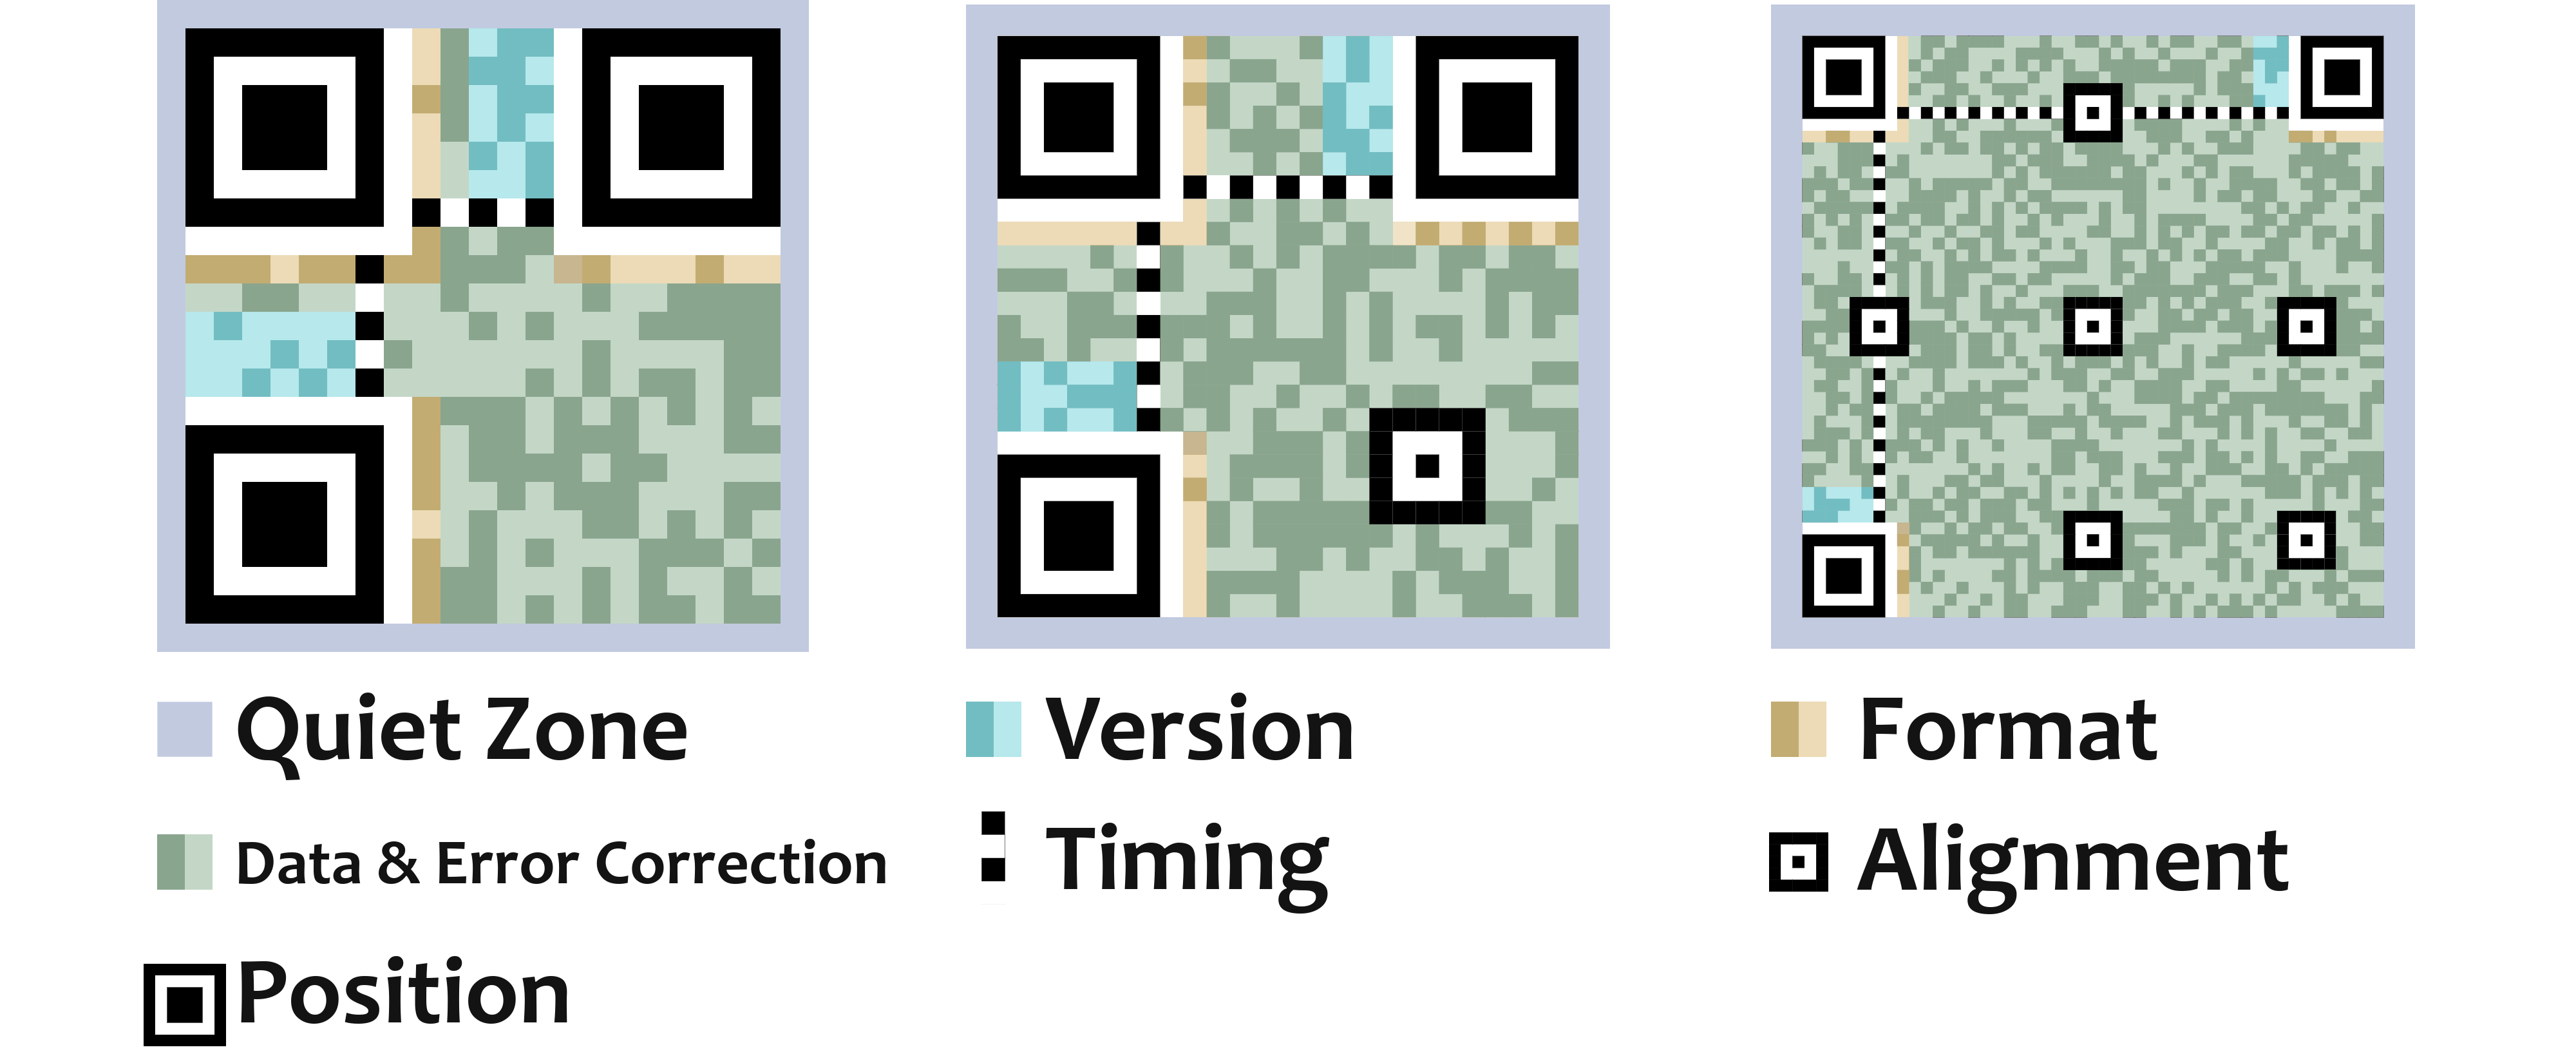
\includegraphics[width=\textwidth]{assets/ch2/QR Codes Figure.png}
	\caption{ These are three QR Codes that store texts. The texts’ lengths get larger going from the left to the right. Notice that the alignment pattern only appears at the bigger QR Codes, and there are multiple ones at the biggest QR Code.}
	\label{QR_code_structure}
\end{figure}

\begin{itemize}
\item \textbf{Quiet Zone:}
This is a white empty area surrounds the QR Code that helps distinguishing it from its surroundings.

\item \textbf{Version Information:} QR Codes have different versions/sizes which specified by these two areas.

\item \textbf{Format Information:}
This part provides details about the error correction level and data mask pattern used.

\item \textbf{Data \& Error Correction:}
This is where both encoded data \& error correction are. data and error correction are stored together enabling the QR code to recover and reconstruct the stored data, even if up to 30\% of the code is damaged or obscured. Data have different types, such as text, URLs, or other. 

\item \textbf{Timing Patterns:}
This part is essential for defining the grid's structure and assists the scanner in establishing the size and coordinate system of the code.

\item \textbf{Alignment Patterns:}
The Alignment Patterns help correct distortion and skewing of the QR code when viewed from different angles. It is especially crucial for larger QR codes that may be prone to bending or misalignment.

\item \textbf{Finder Patterns:}
These patterns assist the scanning device in rapidly locating and orienting the QR code, regardless of its rotation or angle.
\end{itemize}

See \cite{Tiwari2016}, for more information.

\subsection{QR Code Versions and Types}
QR codes come in 40 versions, each representing a different size and data capacity. Version 1 contains 21 × 21 modules, while Version 40 has 177 × 177 modules. As the version number increases, so does the data capacity and the complexity of the code, making it capable of storing more information or supporting higher levels of error correction \cite{Tiwari2016}. 

\begin{figure}[h]
	\centering
	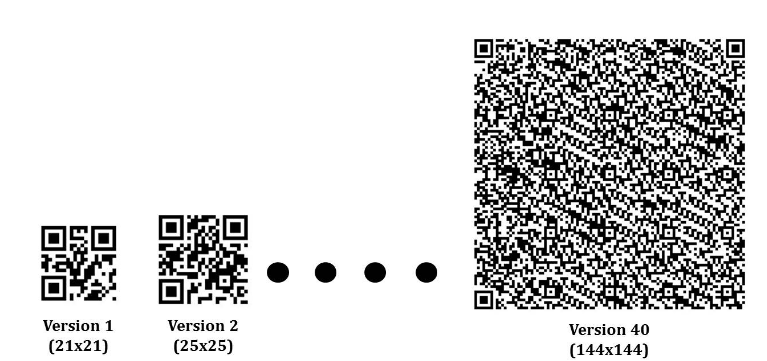
\includegraphics[width=10cm]{assets/ch2/qr_versions}
	\caption{QR codes Versions (adapted from \cite{Tiwari2016}).}
	\label{QR_versions}
\end{figure}


There are also specialized QR code types designed for specific applications:

\begin{itemize}
	\item \textbf{QR Code Model 1 and 2}:
	Model 1 is the original version of the QR code, developed in 1994 by Denso Wave. While model 2 is an improved version of model 1, and it is the one most commonly used today. These models are used for daily basis.
	\item \textbf{Micro QR Code}: Designed to be smaller and simpler, it uses only one Finder Pattern, making it more compact than traditional QR codes. It is often used when space is limited \cite{Tiwari2016}.
	\item \textbf{Logo QR Code}: Allows logos or images to be embedded within the QR code, enhancing the code's visual appeal for marketing or branding purposes \cite{Tiwari2016}.
	\item \textbf{iQR Code}: A flexible matrix-type QR code capable of being printed in various sizes and configurations, from small, high-capacity codes to large codes. It can store more data than standard QR codes and can be inverted or turned into dot patterns for direct part marking \cite{Tiwari2016}.
	\item \textbf{Encrypted QR Code}: Uses encryption techniques to secure the information encoded within, making it suitable for applications requiring data confidentiality \cite{Tiwari2016}.
\end{itemize}

\begin{figure}
	\centering
	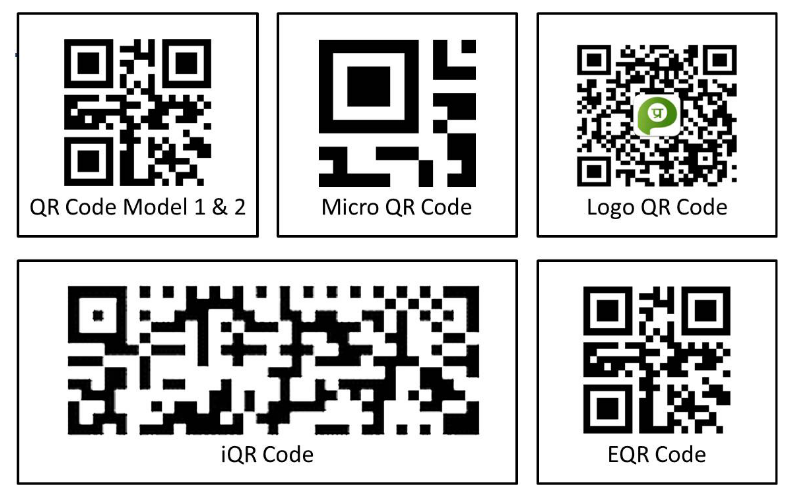
\includegraphics[width=0.7\linewidth]{assets/ch2/qr_codes_type}
	\caption{QR code types (adapted from \cite{Tiwari2016}).}
	\label{qr_code_type}
\end{figure}

\subsection{QR Code Encoding}  
The encoding process for a QR code involves converting data into a matrix of black and white modules. First, the input data is analyzed to determine the appropriate encoding mode, such as numeric, alphanumeric, byte, or Kanji. The data is then transformed into binary code, and error correction is added using Reed-Solomon algorithms, ensuring that the code can still be scanned if partially damaged \cite{Tiwari2016}.

Popular online tools for generating QR codes include:
\begin{itemize}
	\item \textbf{Online Tools}: These free online tools offer simple and fast solutions for both generating and decoding QR codes. QRickit allows users to decode QR codes from uploaded images, while GOQR.me provides various output formats, such as PNG, SVG, and EPS, making it versatile for different use cases \cite{QRCodeMonkey2024}\cite{QRTiger2024}.
	
	
\end{itemize}

For generating QR codes programmatically, popular libraries include:
\begin{itemize}
	\item \textbf{Python - PyQRCode}: A Python library that simplifies QR code creation, allowing output in SVG, PNG, and other formats \cite{PyQRCode2024}.
	\item \textbf{Java - ZXing (Zebra Crossing)}: An open-source library widely used for encoding QR codes in Java and Android applications \cite{ZXing2024}.
	\item \textbf{iOS - Core Image}: iOS provides native QR code generation capabilities via the `CIQRCodeGenerator` filter in the Core Image framework \cite{CoreImage2024}.
\end{itemize}

\subsection{QR Code Decoding}  
\label{qr decode libraries}
Decoding a QR code starts by scanning the Finder Patterns, which allow the scanner to properly align the code. Next, the Format Information is read to apply the correct error correction and mask pattern. Once decoded, the binary data is translated back into the original format (e.g., text, URL) \cite{Tiwari2016}.

Common online tools for decoding QR codes include:
\begin{itemize}
	\item \textbf{Online Tools}: These tools offer versatile QR code decoding solutions across platforms. ZXing is an open-source decoder integrated into Android and web applications, QRickit provides online QR code decoding from uploaded images, and Google Lens allows users to scan and decode QR codes directly via smartphone cameras \cite{ZXing2024, QRickit2024}.
	
\end{itemize}

For decoding programmatically, useful libraries include:
\begin{itemize}
	\item \textbf{Python - Segno}: A versatile Python library for generating and reading both QR and Micro QR codes \cite{Segno2024}.
	\item \textbf{Java - ZXing}: Provides decoding functionality along with encoding, and is widely used for mobile and web apps \cite{ZXing2024}.
	\item \textbf{iOS - AVFoundation}: iOS provides native support for scanning QR codes using the `AVCaptureMetadataOutput` class in the AVFoundation framework \cite{AVFoundation2024}.
	\item \textbf{Google ML Kit}:
	\color{red}temporarily empty...\color{black}
\end{itemize}
 

\section{Indoor Localization}

Indoor localization refers to the process of determining the exact position and orientation of an object or person within indoor environments, where traditional GPS signals are often unreliable. This technology is essential for a wide range of applications, from navigation within large buildings to asset tracking in warehouses.

Various technologies are employed for indoor localization, each with its own strengths and limitations. Wi-Fi, Bluetooth, RFID, and Ultra-Wideband (UWB) are some of the most common methods. While some systems rely on expensive and complex hardware like sensors and Inertial Measurement Units (IMUs), others use more cost-effective solutions such as Bluetooth beacons. The choice of technology often depends on the specific needs of the application, balancing factors such as accuracy, cost, and ease of implementation. For more information, see reference \cite{leitch2023}.

As indoor localization continues to evolve, new techniques and innovative approaches are emerging, including the use of QR codes for precise positioning and tracking. 

\subsection{Indoor Localization with QR Codes}

Indoor localization using QR codes is a method to determine a user’s pose. The system works by strategically placing QR codes around the space—on floors, walls, ceilings, or even hanging panels. Each QR code encodes specific positional information, allowing users to understand their location relative to these codes once they are detected.

\paragraph{Grid Pattern QR codes}

A simple QR-based localization method involves dividing a $n\times m$ meter room into $r$ squares, each with a QR code indicating its exact position. A device, such as a hat with a camera, detects the QR codes as the user moves, determining their location by the square they're in. While this approach provides discrete positional data, it's computationally efficient and useful in contexts like robotics. Although effective for coarse localization, it lacks the precision required for continuous positioning. This approach is used in the solution proposed by \cite{zhang2015}.

\begin{figure}[h] % [h] forces the figure to be placed exactly here in the text
	\centering
	\includegraphics[width=5cm]{example-image-A}
	\caption{Grid Patter Illustration}
	\label{grid_pattern_illustration}
\end{figure}



\paragraph{Pose Estimation with QR codes}

Another approach of indoor localization involves calculating the relative position and orientation (pose) of the QR code in relation to the camera. After detecting a QR code, the camera determines its position and orientation relative to itself, and by combining this information with the known global position of the QR code, the system can estimate the user’s precise, continuous position within the space. Although this method offers significantly higher positional accuracy, it requires more computational resources, as it involves additional steps such as camera calibration to determine intrinsic parameters. This added complexity makes it more resource-intensive compared to grid-based localization, but it delivers continuous localization with greater precision. \textcolor{red} {Cite the papar that use this approach}

\begin{figure}[h] % [h] forces the figure to be placed exactly here in the text
	\centering
	\includegraphics[width=5cm]{example-image-A}
	\caption{Grid Patter Illustration}
	\label{pose_estimation_illustration}
\end{figure}


In a well-designed setup, the system's effectiveness remains high, irrespective of the QR codes’ locations. By tailoring the placement and setup of QR codes to suit the environment, the system can deliver robust indoor localization, whether it prioritizes simplicity or precision.
\section{Application Programming Interface}

An Application Programming Interface (API) is a set of rules that allows different software applications to communicate with each other. It defines the methods and data formats that applications can use to request and exchange information, simplifying the process for developers to build compatible software. For instance, when using a social media login to access a new app, an API handles the authentication process.

APIs are essential in various technology domains, including web and mobile applications, where they enable diverse services to work together seamlessly. For example, a travel booking website may utilize APIs to aggregate data from various airline and hotel services, allowing users to compare prices and availability in one place. Similarly, a weather app may leverage APIs to retrieve real-time weather data from different sources, providing accurate forecasts based on user location \cite{ibm2024}.


\textbf{Base URL:} The base URL is the starting point for accessing an API. It usually includes the protocol (like HTTP or HTTPS) and the domain name where the API is hosted. For example, if the base URL is \texttt{https://api.example.com}, all API requests will start from this address.

\textbf{Endpoints:} Endpoints are specific paths added to the base URL that direct requests to particular resources or functions within the API. For example, if you want to access user data, you might use an endpoint like \texttt{/users}. The full URL for this request would be \texttt{https://api.example.com/users}.

\textbf{HTTP Methods:} APIs commonly use HTTP methods to specify the action to be performed. The most common methods are:
\begin{itemize}
	\item \texttt{GET}: Retrieve data from the server.
	\item \texttt{POST}: Send new data to the server.
	\item \texttt{PUT}: Update existing data on the server.
	\item \texttt{DELETE}: Remove data from the server.
\end{itemize}
 
 \textcolor{blue}{
 	\begin{itemize}
 		\item ADD frameworks example, including what will be used in the next semester.
 \end{itemize}}


\section{Databases}

A \textbf{database} is an organized system for storing, retrieving, and managing data. It enables efficient data handling, storage, and access for various applications, from small personal projects to large-scale enterprise solutions. Databases are essential for maintaining consistency, accuracy, and accessibility in data storage. They use structures such as tables to organize data into columns (fields) and rows (records). Two common key elements in databases are \textbf{Primary Keys (PK)} and \textbf{Foreign Keys (FK)}. The Primary Key uniquely identifies each record within a table, ensuring that data remains unique, while the Foreign Key links tables, establishing relationships between them to enforce data integrity.

There are various types of databases, including:
\begin{itemize}
	\item \textbf{Relational Databases} – Organize data into tables and use structured query language (SQL) for data manipulation. Examples include MySQL, PostgreSQL, and SQLite.
	\item \textbf{NoSQL Databases} – Store unstructured data, often in formats like JSON. They are designed for scalability and high performance in handling large datasets, as in MongoDB and Cassandra.
\end{itemize}

\subsection{Entity-Relationship Diagram (ERD)}
The \textbf{Entity-Relationship Diagram (ERD)} is a visual representation of the data model for a system. It illustrates the entities involved, their attributes, and the relationships between them. Each entity corresponds to a table in the database, while attributes represent the fields within those tables. Relationships indicate how entities interact, showcasing cardinality (e.g., one-to-many or many-to-many) and participation (e.g., optional or mandatory). The ERD serves as a crucial tool in the design phase, promoting clear communication about the data structure and its constraints.


\begin{figure}[h]
	\centering
	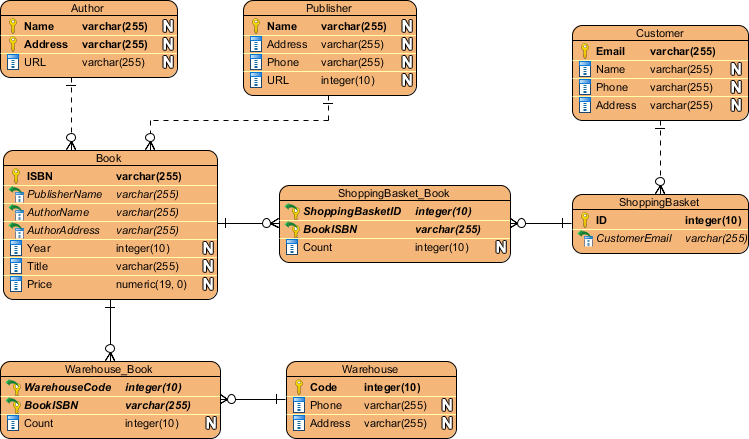
\includegraphics[width=0.9\linewidth]{assets/ch2/ERD}
	\caption{This ERD, adapted from \cite{visual-paradigm}, represents a bookstore database, with entities like Author, Publisher, Book, Warehouse, Customer, and ShoppingBasket. It shows relationships between entities, such as customers adding books to shopping baskets and warehouses storing book inventory, linked by primary and foreign keys.}
	\label{fig:erd}
\end{figure}


\subsection{Structured Query Language (SQL)}
\textbf{SQL (Structured Query Language)} is the standard language used to interact with relational databases. SQL provides commands for data insertion, query, updating, and deletion. It also includes commands for schema creation and modification. Some fundamental SQL commands include:

\begin{itemize}
	\item \texttt{SELECT} for retrieving data,
	\item \texttt{INSERT} for adding new data,
	\item \texttt{UPDATE} for modifying existing data,
	\item \texttt{DELETE} for removing data,
	\item \texttt{CREATE TABLE} for defining new tables,
	\item \texttt{JOIN} for combining data from multiple tables.
\end{itemize}

SQL enables efficient, standardized access to data, supporting complex queries and data manipulation tasks.

\subsection{SQLite3}
\textbf{SQLite3} is a lightweight, serverless, and self-contained relational database engine, commonly used for applications requiring minimal configuration and overhead. Unlike other SQL databases, SQLite does not require a separate server process. Instead, it stores data in a single file, making it highly portable and simple to integrate. SQLite is ideal for embedded systems, mobile apps, and small to medium-scale projects due to its reliability, compact size, and ease of use.

\section{Customizable Guidance}
The customizable guidance system guides blind and visually impaired people navigating through indoor environments. This can be done by reading on user specific information or instructions based on their locations in the buildings. This system also can guide the users by assisting them following a path to their desired destinations.

\section{Objects Detection}
A goal of computer vision that tasks a device to identify an object via unique attributes such it's silhouette and perceived shape while accounting illumination and the viewpoint of it and classify it under known predefined categories (such as a car or a trash can) then put a rectangle called a bounding box indicating the name of an object and it's size relative to the  perspective of the pupil of the device.

The approaches that will be covered are: Deformable Parts Model (DPM), R-CNN (Regional Convoluted Neural Networks), and YOLO (You Only Look Once).

\subsection{Deformable Parts Model}
The main idea of this method is objects are the sum of their parts, with separate dedicated filters for each of the machines employed, these filters are:

\begin{itemize}
\item \textbf{coarse root filter:} tasked to detect the silhouette of the object without taking
into account the parts.
\item \textbf{parts filter:} each distinguishable feature of the silhouette grouped together.
\item \textbf{Spatial filter model:} Indicates the location of each part in relation to the root.
\end{itemize}

These filters then feed to the next one in order to end up in a Support Vector Machine (SVM) to decide which object it can be classified under. This method doesn't consider speed or the computational power of the device, which results in it demanding very a capable parallel processor such as a GPU (Graphical Processing Unit) and takes a significant amount of time, thus not being qualified for real-time applications.

\subsection{Regonal-CNN}
\color{red}Temporarily empty...\color{black}

\subsection{You Only Look Once}
Opposite to all the above methods, YOLO only views the image once by basing all of the calculations on a single image, eliminating the need of multiple, parallel proc-esses running together which ultimately reduces time wasted on a single calculation. The algorithm takes a two-dimensional input image from a given source, overlay an evenly-spaced square with dimensions n x n on each of the two axis, then take the  bounding boxes present in the grid and the confidence map, where it determines which of the objects in the cells are and categorize them to finally be combined, resulting in a list of detections it made. [REFERENCE IMAGE HERE] It's capable of being put in real-time applications thanks to it's efficiency and low data-processing. See reference [num] for more details.
\section{Camera Module}

Camera modules have become integral components in various embedded systems, enabling devices to capture images and video for processing and analysis. These modules are typically made up of an image sensor, lens, and support circuitry, which allow them to interface with microcontrollers, single-board computers, and other embedded platforms. Camera modules are often classified based on their resolution, power consumption, compatibility with specific devices, and imaging quality. The OV series of camera modules from OmniVision, a prominent supplier of CMOS image sensors, are particularly popular in applications ranging from surveillance to IoT and computer vision. Below, we discuss three widely used models: the OV2640, OV7670, and OV5640.

\subsection{OV2640}
The OV2640 is a compact, low-power camera module with a 2-megapixel (1600 x 1200 pixels) CMOS sensor. This module is widely used in embedded applications due to its energy efficiency and compatibility with microcontrollers, particularly the ESP32. The OV2640 supports image output formats like JPEG, YUV, and RGB, making it versatile for different applications. It operates effectively at lower resolutions, allowing faster processing and reduced memory usage, which is essential in IoT devices that require minimal power. Additionally, the OV2640 includes support for automatic white balance, exposure control, and other image enhancements, allowing it to capture acceptable quality images in various lighting conditions.\cite{OV2640}
\begin{figure}[h]
	\centering
	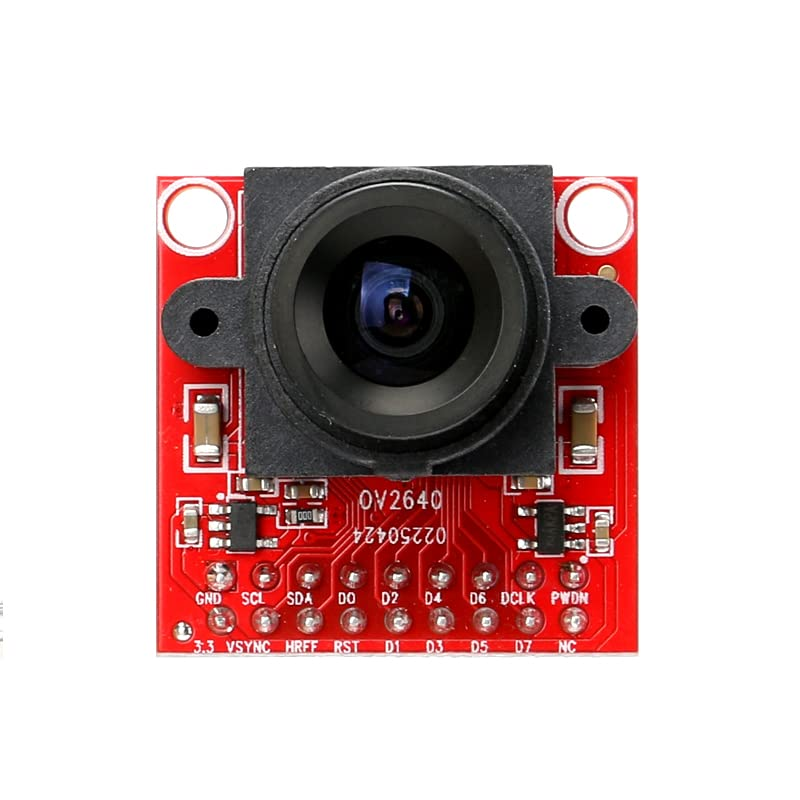
\includegraphics[width=0.5\linewidth]{assets/ch2/OV2640}
	\caption{OV2460 Camera Module}
	\label{fig:ov2640}
\end{figure}


\subsection{OV7670}
The OV7670 is a low-cost VGA (640 x 480 pixels) camera module often chosen for applications requiring basic image capture, particularly where high resolution is not a priority. With its 0.3-megapixel sensor, the OV7670 is suitable for simpler image processing tasks, such as color tracking, object detection, and line following, often found in educational and hobbyist projects. The OV7670 is compatible with many microcontrollers, like the Arduino, due to its relatively low data and power requirements. Although it lacks some of the advanced features found in newer modules, it still offers functionalities such as image scaling, automatic white balance, and gamma correction, making it a viable choice for cost-sensitive and low-power applications. \cite{OV7670}
\begin{figure}[h]
	\centering
	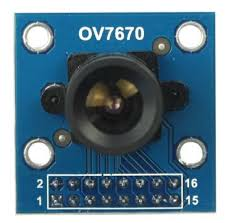
\includegraphics[width=0.5\linewidth]{assets/ch2/OV7670}
	\caption{OV7670 Camera Module}
	\label{fig:ov7670}
\end{figure}


\subsection{OV5640}
The OV5640 is a high-resolution camera module with a 5-megapixel (2592 x 1944 pixels) CMOS sensor. It is favored for applications requiring detailed images, such as facial recognition, barcode scanning, and other computer vision tasks. This module provides a range of image formats, including JPEG, RAW, and YUV, and supports video output at different frame rates, depending on the resolution. The OV5640 also features advanced imaging controls like autofocus, which can enhance the clarity and quality of images in diverse environments. Due to its higher resolution and additional features, the OV5640 requires more processing power and memory, making it suitable for platforms like Raspberry Pi and other single-board computers capable of handling high-definition image processing. \cite{OV5640}

\begin{figure}[h]
	\centering
	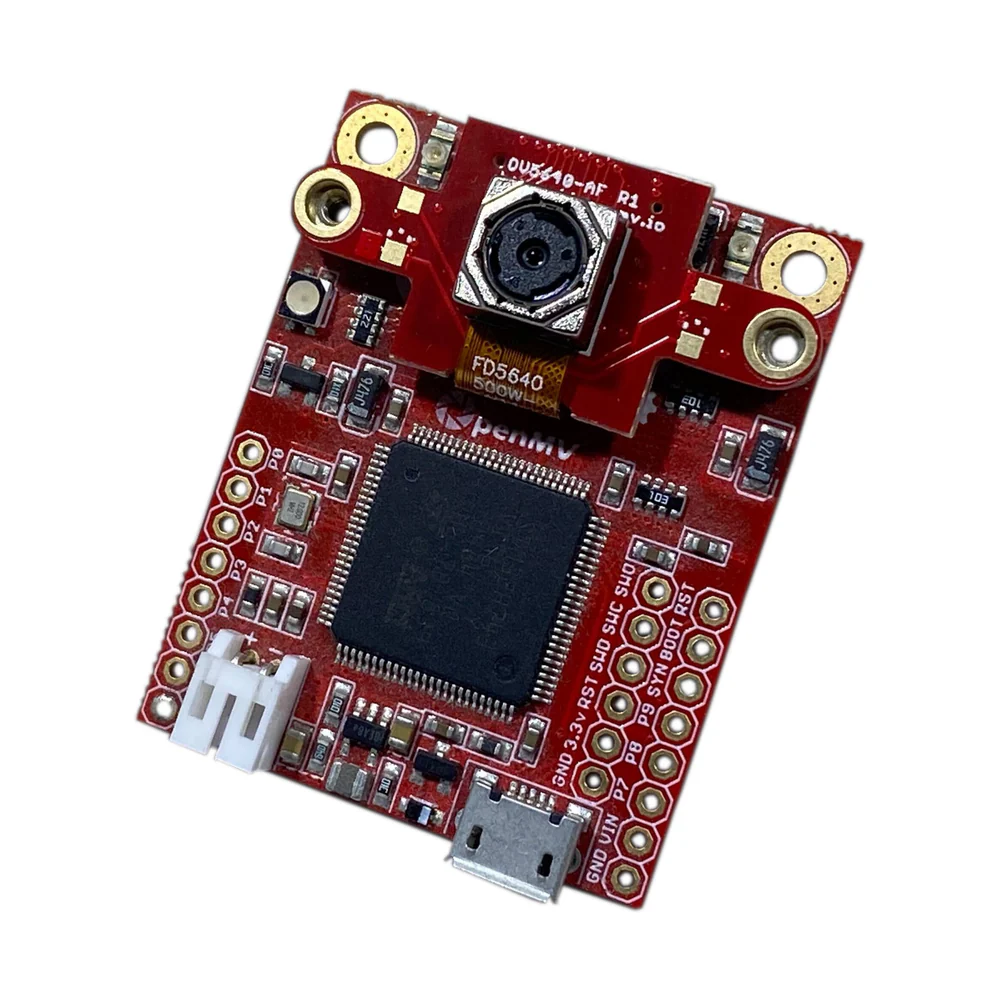
\includegraphics[width=0.5\linewidth]{assets/ch2/OV5640}
	\caption{OV5640 Camera Module}
	\label{fig:ov5640}
\end{figure}




\section{Audio Amplification Modules \& Speakers}

An audio module is an electronic device designed to amplify and process audio signals, allowing for the playback of sound in various applications. Speakers are transducers that convert electrical energy into sound energy, enabling us to hear audio signals. Together, audio modules and speakers create a complete audio playback system, necessary for applications ranging from personal electronics to professional sound systems.

\subsection{Speakers}

Speakers are devices that convert electrical signals into sound waves. They are classified into various types based on their design and application. Two common types of speakers include:

\begin{itemize}
	\item \textbf{Dynamic Speakers}: These are the most common type, using a voice coil and magnet to produce sound.
	\item \textbf{Subwoofers}: Specialized speakers designed to reproduce low-frequency sounds (bass), providing depth to the audio experience.
\end{itemize}

\subsection{Audio Modules}

Audio modules are compact devices designed to amplify audio signals and can include additional features like Bluetooth connectivity, equalization, and noise reduction. Some notable audio modules include:

\begin{figure}[h!]
	\centering
	\begin{subfigure}[b]{0.22\textwidth}
		\centering
		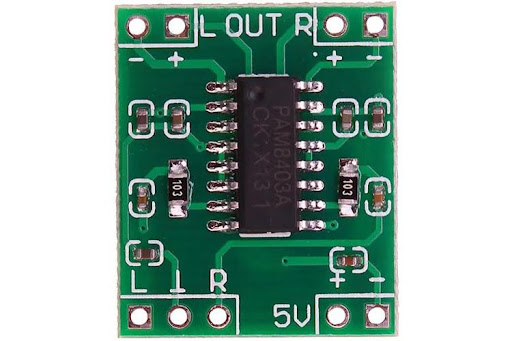
\includegraphics[width=\textwidth]{assets/ch2/PAM8403}
		\caption{}
		\label{fig:pam8403}
	\end{subfigure}
	\hfill
	\begin{subfigure}[b]{0.22\textwidth}
		\centering
		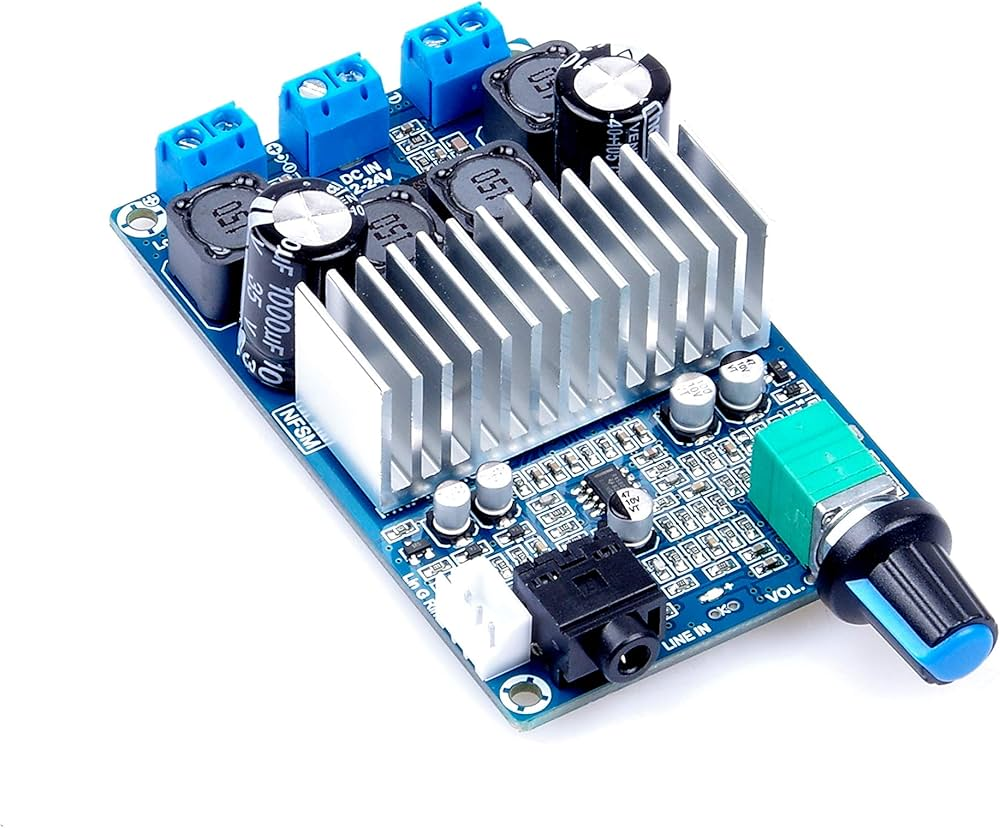
\includegraphics[width=\textwidth]{assets/ch2/TPA3116D2}
		\caption{}
		\label{fig:tpa3116d2}
	\end{subfigure}
	\hfill
	\begin{subfigure}[b]{0.22\textwidth}
		\centering
		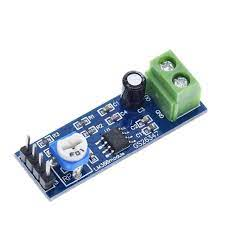
\includegraphics[width=\textwidth]{assets/ch2/LM386}
		\caption{}
		\label{fig:lm386}
	\end{subfigure}
	\hfill
	\begin{subfigure}[b]{0.22\textwidth}
		\centering
		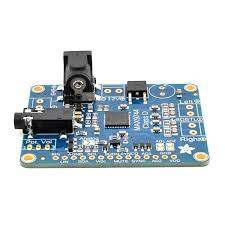
\includegraphics[width=\textwidth]{assets/ch2/MAX9744}
		\caption{}
		\label{fig:max9744}
	\end{subfigure}
	\caption{Audio Amplification Modules: (a) PAM8403, (b) TPA3116D2, (c) LM386, and (d) MAX9744.}
	\label{fig:audio_modules}
\end{figure}

\begin{itemize}
	\item \textbf{PAM8403}: A popular audio amplifier module known for its efficiency and compact size, suitable for small audio projects.
	
	
	\item \textbf{TPA3116D2}: A powerful audio amplifier capable of delivering higher output power, often used in larger audio systems.
	
	
	
	\item \textbf{LM386}: A low-power audio amplifier that is easy to use and perfect for basic applications.
	
	
	\item \textbf{MAX9744}: A high-efficiency audio amplifier designed for demanding audio applications, providing high-quality sound output.
	
	
\end{itemize}

\section{ESP32}

Embedded System Processors (ESP) are versatile microcontroller units (MCUs) widely used in Internet of Things (IoT) and embedded applications. Developed by Espressif Systems, these modules combine powerful processing with Wi-Fi and Bluetooth connectivity, making them ideal for smart home devices, wearables, and industrial automation.

\begin{figure}[h!]
	\centering
	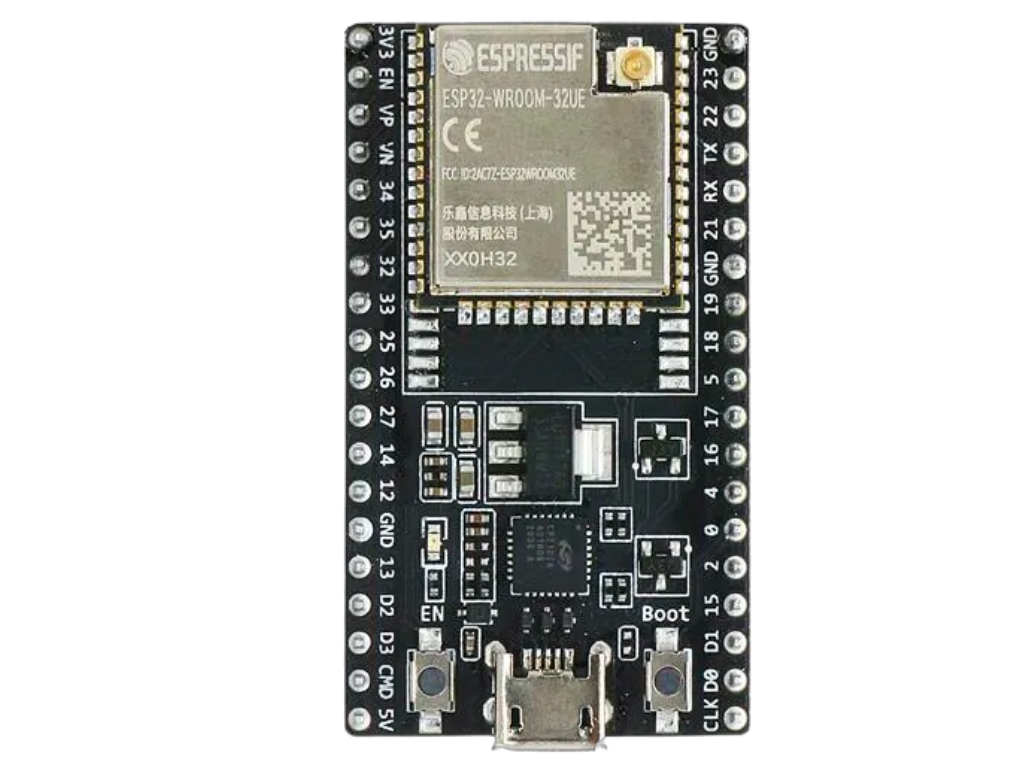
\includegraphics[width=0.4\linewidth]{assets/ch2/esp32}
	\caption{ESP32-WROOM Development board}
	\label{fig:esp32}
\end{figure}

\subsection{ESP Series Overview}

The ESP series includes different models tailored to specific application needs for performance, power efficiency, and connectivity. Key types include:

\begin{itemize}
	\item \textbf{ESP8266 Series:} A cost-effective option with a 32-bit LX6 single-core processor (up to 160 MHz), supporting 2.4 GHz Wi-Fi and peripheral interfaces like UART, I2C, and PWM. Its low power consumption suits battery-powered applications.
	
	\item \textbf{ESP32 Series:} Offers more power and connectivity. The ESP32-S2 has a single-core LX7 processor, while the ESP32-S3 features a dual-core LX7 processor (up to 240 MHz), with 2.4 GHz Wi-Fi and Bluetooth 5.0. It includes security features like secure boot and flash encryption.
	
	\item \textbf{ESP32-S2 Series:} A low-power option with a single-core LX7 processor (up to 240 MHz) and Wi-Fi support. It includes USB OTG and advanced security features, making it suitable for secure IoT applications.
	
	\item \textbf{ESP32-S3 Series:} Designed for AI and neural network applications, it features a dual-core LX7 processor (up to 240 MHz), with Wi-Fi and Bluetooth 5 (LE). It has added vector instructions for AI tasks and comprehensive security options.
\end{itemize}

\subsection{Key Features of ESP Modules}

ESP modules provide a range of features for various applications:

\begin{itemize}
	\item \textbf{Processing Power:} 32-bit processors with single or dual cores, running between 160 and 240 MHz.
	
	\item \textbf{Wireless Connectivity:} All modules support 2.4 GHz Wi-Fi; some also include Bluetooth 5.0 (LE).
	
	\item \textbf{Memory and Storage:} Includes SRAM and ROM, with options to add external flash and PSRAM. The ESP32-S3, for instance, has up to 512 KB SRAM and supports various SPI interfaces.
	
	\item \textbf{Peripherals and Interfaces:} Offers GPIO, SPI, I2C, I2S, UART, PWM, ADC, DAC, and USB OTG (on select models), supporting a wide variety of sensors and devices.
	
	\item \textbf{Power Efficiency:} Low-power modes and fine-grained control make ESP modules suitable for battery-powered devices, with the ESP32-S2 optimized for ultra-low-power applications.
\end{itemize}

With their range of types, processors, and features, ESP modules offer a flexible solution for IoT and embedded systems, meeting the needs of modern, connected applications.

\section{Related Work}

Navigation solutions for visually impaired individuals utilize a range of technologies, including Bluetooth Low Energy (BLE), LiDAR, and artificial landmarks. Each of these technologies offers unique advantages and limitations that impact their effectiveness in real-world applications. In this section, we explore different solutions that incorporate various technological approaches, highlighting how each addresses the challenges faced by visually impaired users in navigating indoor environments.

PathFinder, proposed by Kuribayashi et al. \cite{kuribayashi2023}, is a map-less navigation system developed to assist blind individuals in navigating unfamiliar indoor environments. Unlike other systems that rely on prebuilt maps, PathFinder uses real-time detection of intersections and signs to guide users. The system includes a suitcase-shaped robot that blind users control through a handle interface, receiving audio feedback about their surroundings. PathFinder’s core navigation capabilities are powered by LiDAR for detecting intersections and image processing via a high-resolution camera to recognize directional and textual signs. Developed using a participatory design approach with blind users, the system focuses on addressing the most relevant challenges of navigating unknown spaces. In a user study involving seven blind participants, PathFinder demonstrated significant effectiveness in helping users navigate unfamiliar environments with greater confidence than when using traditional aids like canes or guide dogs. Despite requiring more user effort than map-based systems, participants appreciated PathFinder’s flexibility and adaptability to environments without prior mapping. The study concluded that PathFinder offers a valuable solution for blind individuals, particularly in situations where prebuilt maps are unavailable.

Ahmetovic et al. \cite{ahmetovic2016} presents NavCog, NavCog is a smartphone-based navigation system designed to help visually impaired individuals with turn-by-turn guidance in indoor and outdoor environments. The system uses Bluetooth Low Energy (BLE) beacons for accurate localization, employing a K-nearest neighbor (KNN) algorithm to compare current signal strengths with previously recorded beacon signal fingerprints. NavCog provides real-time auditory navigation instructions to guide users along a predetermined path and also notifies them of nearby points of interest (POI) and accessibility issues such as stairs or obstacles.

One of NavCog's key features is its ability to be easily deployed in large, complex environments without requiring significant infrastructure modifications. In a study conducted with six visually impaired participants on a university campus, NavCog successfully guided users through both familiar and unfamiliar spaces, receiving positive feedback on its navigation features. The study emphasizes NavCog’s flexibility and ease of use, making it a promising tool for visually impaired individuals navigating new environments.


The work by Fraga et al. \cite{fraga2022} presents an indoor navigation system has been developed for visually impaired individuals. This system uses QR code markers and computer vision techniques to provide real-time navigation instructions. Users scan QR codes placed in different locations to receive guidance along optimal paths. The system cross-references the scanned information with a prebuilt database. Audio feedback informs users of their current location and the next steps in the navigation process. If the user deviates from the planned route, the system recalculates the path. Importantly, this system does not require internet connectivity, making it practical for offline use. Additionally, the system includes a collision avoidance feature based on a monocular depth estimation algorithm, which predicts distances to obstacles using 2D images. Experimental results in a controlled environment demonstrated that the system accurately guided users and effectively detected obstacles with acceptable depth estimation margins. This study highlights the potential of QR code-based navigation for enhancing mobility for visually impaired individuals and suggests future integration into smartphones or AI accelerators for improved usability.


In conclusion, our solution distinguishes itself by employing a cost-effective navigation tool that requires only a standard smartphone. This straightforward approach minimizes the need for additional hardware, thereby increasing accessibility for users. Unlike systems such as PathFinder and NavCog, which depend on specialized technologies like LiDAR and Bluetooth beacons, our method aims to simplify navigation by leveraging existing smartphone capabilities. Furthermore, it's easy to integrate optional remote or Wi-Fi cameras to enhance the navigation experience without imposing significant costs. Our primary objective is to deliver a practical and user-friendly solution specifically tailored for visually impaired individuals, ensuring ease of use in real-world.



In conclusion, our solution distinguishes itself by utilizing QR codes not only for localization, but as well for storing navigation instructions. Unlike systems like PathFinder and NavCog, which depend on specialized technologies such as LiDAR and BLE beacons, our approach is designed to operate with minimal hardware requirements, relying solely on a standard smartphone. Also, external hardware can be integrated to the system for more convenient. Additionally, the system comes with an intuitive dashboard that empowers building managers to generate and manage QR codes effortlessly, facilitating seamless integration into diverse indoor environments. This approach ensures affordability, scalability, and accessibility, making it a user-friendly and cost-effective solution tailored to the needs of visually impaired individuals.



% ========= BEGIN: CHAPTER-3 ======== %
\chapter{Methodology}
\newpage
\section{System Architecture Overview}

This section provides an overview of the architecture of our indoor navigation system, designed to assist visually impaired users with real-time, context-aware guidance within indoor environments. The system leverages a combination of mobile technology, backend services, and sensory input devices to deliver seamless and accessible navigation. Below, we present the key components, data flow, technology stack, and a system diagram to illustrate the complete structure of the system.

\subsection{High-Level View of Components}

The system is composed of several interacting components:

\begin{itemize}
	\item \textbf{Mobile Application}: The main user interface for visually impaired users. This application handles QR code scanning, voice command processing, navigation feedback (both audio and vibration), and integration with external devices (e.g., camera, microphone).
	\item \textbf{QR Code Scanner and Object Detection}: The mobile app uses a camera sensor connected to an ESP32 microcontroller to scan QR codes and detect key objects, such as trashcans and chairs, within the environment. YOLOv10 is employed for efficient object detection, while Google’s ML Kit is used for QR code scanning.
	\item \textbf{Navigation and Guidance System}: This module within the mobile application provides real-time navigation assistance based on the user’s location, direction, and desired destination. It uses data from QR codes and object detection to inform users about nearby obstacles and paths.
	\item \textbf{Backend and Database}: A cloud-based backend server and database store user and navigation data, such as QR code global positions, custom instructions, and map layouts. The server processes requests for location-specific information and delivers relevant navigation instructions to the app.
	\item \textbf{I/O Devices and ESP32 Microcontroller}: An ESP32 microcontroller manages additional components, including a camera module for QR code scanning, an ultrasonic sensor for obstacle detection, and a speaker for audio output. The ESP32 also transmits audio and tactile feedback to guide users.
\end{itemize}

\subsection{Data Flow}

The system’s data flow is designed for efficient and seamless interactions across components. Below is an outline of the primary data flow:

\begin{enumerate}
	\item \textbf{QR Code Scanning and Localization}: The camera captures a frame containing a QR code, which the app decodes using ML Kit. The app then retrieves the global position of the QR code from the backend, which provides a reference point for the user’s current location.
	\item \textbf{Navigation Instruction Retrieval}: After the QR code is decoded, the mobile app queries the backend for location-specific instructions, which are returned in real-time and provided to the user as audio guidance.
	\item \textbf{Voice Command Processing}: Users can interact with the navigation system via voice commands. The app processes these commands locally and may query the backend if needed for contextual information (e.g., “Guide me to the nearest exit”).
	\item \textbf{Object Detection and Proximity Alerts}: The ESP32 detects nearby obstacles using the ultrasonic sensor and sends alerts to the mobile app, which provides vibration feedback to notify users.
	\item \textbf{Customizable Guidance Updates}: When users reach specific points (QR codes or predefined milestones), the app provides updated instructions tailored to the current context, based on backend data.
\end{enumerate}

\subsection{Technology Stack}

The following tools and technologies were selected for each component of the system:

\begin{itemize}
	\item \textbf{Mobile Application Development}: Developed using Kotlin.
	\item \textbf{QR Code Scanning and Object Detection}: Google ML Kit is used for QR code detection and decoding, while YOLOv10 (converted to TensorFlow Lite) performs real-time object detection.
	\item \textbf{Navigation and Guidance Logic}: Implemented with OpenCV for pose estimation and CameraX for real-time camera access.
	\item \textbf{Backend and Database}: SQLite3 for lightweight database, FastAPI for quick and easy to deploy API, Python for other services such as QR code generation. 
	\item \textbf{ESP32 Microcontroller and Sensors}: The ESP32 is programmed to control the camera, ultrasonic sensor, and speaker, utilizing TensorFlow Lite for lightweight operations on embedded devices.
\end{itemize}







\section{Backend Infrastructure}

The backend infrastructure serves as the foundational framework for our system, managing data storage, processing requests, and delivering instructions in response to QR code scans. It is essential for the functionality of various components, ensuring accurate and timely responses to user interactions. For instance, the localization system relies on the backend to calculate global positions, while the customizable guidance system utilizes it to retrieve the latest instructions tailored for users. Each part of the system depends on the backend to keep data accurate and up-to-date. The backend is composed of the following components:
\subsection{Database}

The database serves as the backbone of the system, storing all data related to QR codes, building layouts, and navigation instructions. It is designed to organize QR code data in a manner that ensures each QR code is uniquely identifiable, allowing the mobile application to efficiently retrieve the correct information upon each scan.

\begin{figure}[h]
	\centering
	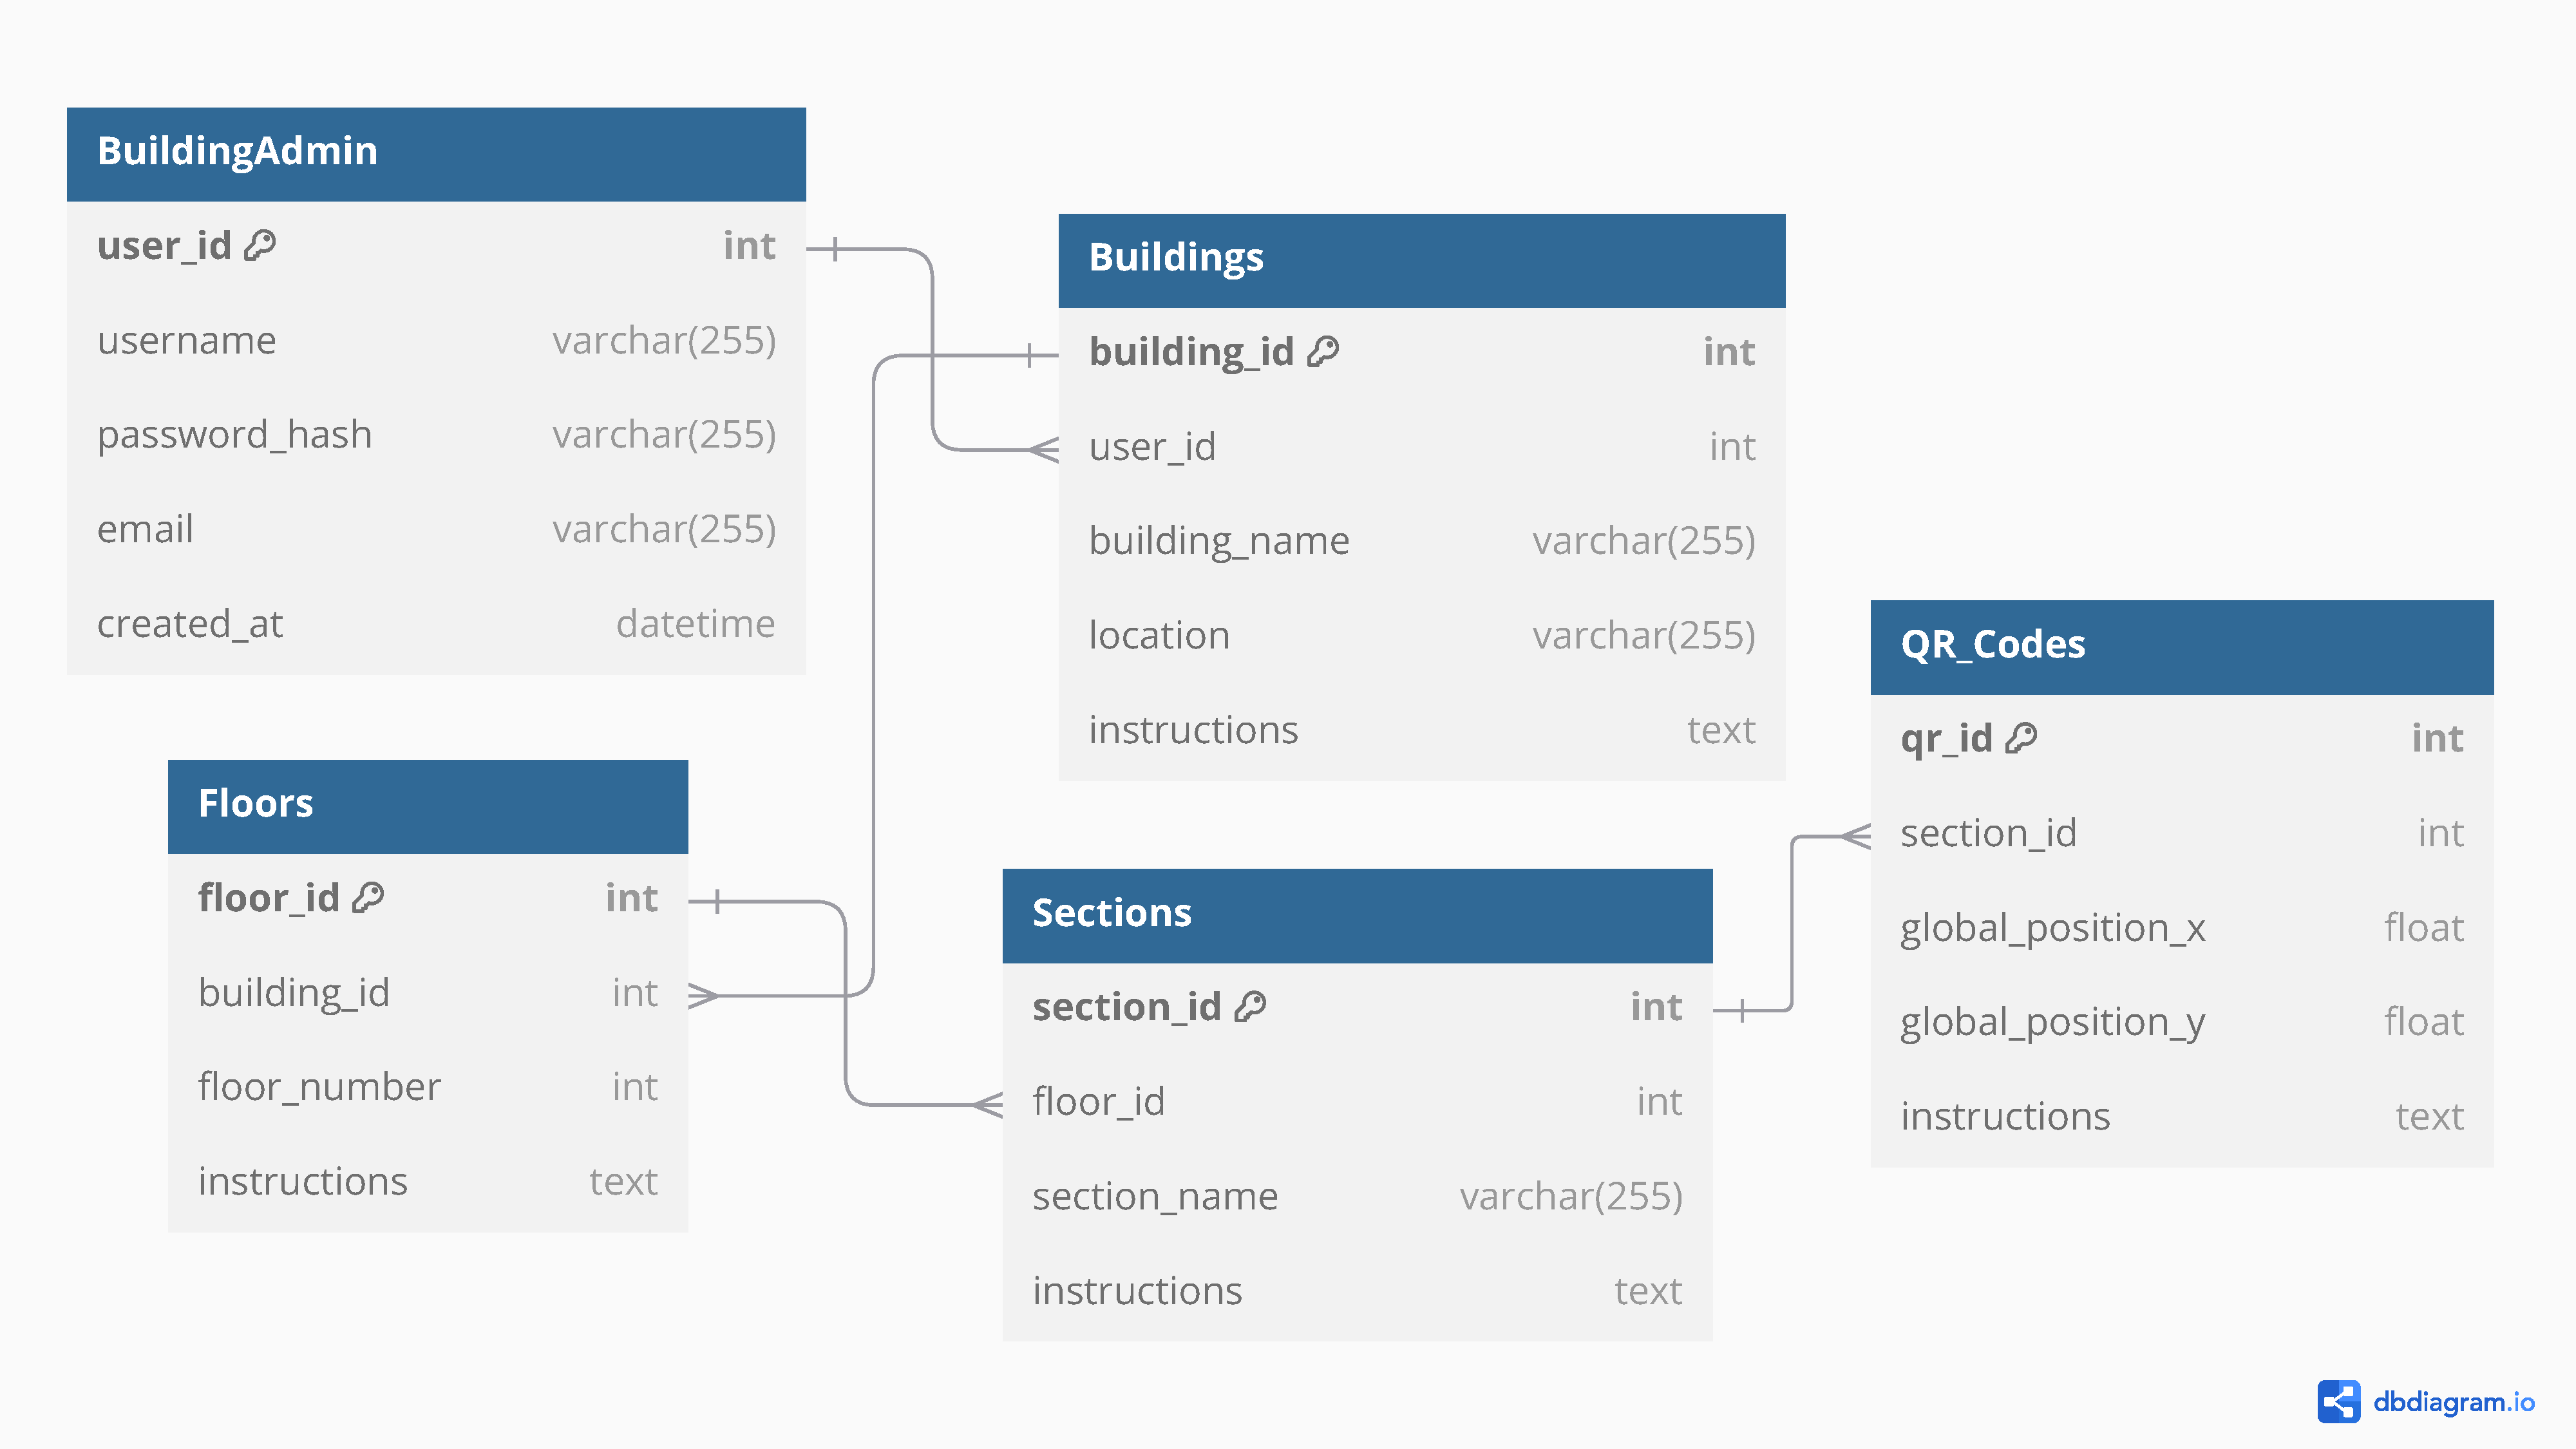
\includegraphics[width=1\linewidth]{assets/ch3/our_ERD}
	\caption{This Entity-Relationship Diagram (ERD) of Mosaned database}
	\label{fig:our_ERD}
\end{figure}

\subsection{Table: BuildingAdmin}  
\begin{itemize}
	\item \textbf{user\_id (Primary Key)}: A unique identifier for each user of the system, enabling individual management of buildings and associated data.
	\item \textbf{username}: The name chosen by the user for login purposes.
	\item \textbf{password\_hash}: A secure hash of the user's password used for authentication.
	\item \textbf{email}: The user's email address, utilized for notifications and account recovery.
	\item \textbf{created\_at}: A timestamp indicating when the user account was created.
\end{itemize}

\subsection{Table: Buildings}  
\begin{itemize}
	\item \textbf{building\_id (Primary Key)}: A unique identifier for each building within the system.
	\item \textbf{user\_id (Foreign Key)}: Links the building to the associated user in the \texttt{BuildingAdmin} table, ensuring that each building is managed by the correct user.
	\item \textbf{building\_name}: The name of the building.
	\item \textbf{location}: The physical address or description of the building's location.
	\item \textbf{instructions}: General instructions related to the building, providing contextual information for navigation and management.
\end{itemize}

\subsection{Table: Floors}  
\begin{itemize}
	\item \textbf{floor\_id (Primary Key)}: A unique identifier for each floor within a building.
	\item \textbf{building\_id (Foreign Key)}: Associates the floor with its corresponding building, establishing a clear hierarchical structure.
	\item \textbf{floor\_number}: Indicates the number of the floor (e.g., 1 for the first floor, 2 for the second, etc.).
	\item \textbf{instructions}: Specific instructions related to that floor, assisting users with effective navigation.
\end{itemize}

\subsection{Table: Sections}  
\begin{itemize}
	\item \textbf{section\_id (Primary Key)}: A unique identifier for each section on a floor.
	\item \textbf{floor\_id (Foreign Key)}: Links the section to its respective floor, maintaining the organizational hierarchy.
	\item \textbf{section\_name}: The name or description of the section within the floor.
	\item \textbf{instructions}: Instructions specific to the section, enhancing the user’s ability to navigate the area.
\end{itemize}

\subsection{Table: QR\_Codes}  
\begin{itemize}
	\item \textbf{qr\_id (Primary Key)}: A unique identifier for each QR code, ensuring no duplicates exist within the system.
	\item \textbf{section\_id (Foreign Key)}: Connects the QR code to its specific section.
	\item \textbf{global\_position\_x}: The X-coordinate representing the global position of the QR code.
	\item \textbf{global\_position\_y}: The Y-coordinate indicating the QR code's position, further aiding in navigation.
	\item \textbf{instructions}: Specific instructions directly linked to the QR code, providing targeted guidance for users when the QR code is scanned.
\end{itemize}




\subsection{Application Programming Interface (API)}

The API serves as the bridge between the mobile app, the database, and the building management dashboard. Its primary responsibilities are:
\begin{itemize}
	\item \textbf{Data Retrieval and Delivery:} When a QR code is scanned, the API retrieves the associated information from the database and sends it to the mobile app for processing.
	\item \textbf{Instruction Updates:} The API also handles data updates from the dashboard, ensuring the latest QR code instructions are accessible to users in real time.
	\item \textbf{User Authentication:} Manages secure access to both the dashboard and the mobile app, allowing only authenticated users to modify or retrieve data.
\end{itemize}

\textcolor{blue}{
	\begin{itemize}
		\item ADD one example of API Endpoints, and the rest on Appendix 
\end{itemize}}

\subsection{Web Server}

The Web Server hosts the building management dashboard and processes web requests, allowing administrators to view and manage QR code data and building layouts. It communicates with the API to send updates to the database and deliver real-time data to the mobile app. 

\textcolor{blue}{
	\begin{itemize}
		\item ADD What tools/framework used to host the dashboard on 3.6
\end{itemize}}



\section{Mobile Application}

The Mobile Application serves as the primary interface for visually impaired users, offering intuitive features that facilitate navigation in indoor environments. Designed with accessibility in mind, the app implements both the customizable guidance and localization systems, ensuring that users receive accurate and real-time navigation assistance.

The application functionality includes:

\begin{itemize}
	\item \textbf{QR Code Scanning:} The app’s camera detects and decodes QR codes, automatically initiating the customizable guidance system. Upon scanning a QR code, the application identifies its unique ID, which is crucial for retrieving the corresponding navigation instructions from the central database.
	
	\item \textbf{Customizable Guidance Imp.:} 
	
	
	\item \textbf{Localization Imp.:} 
	
	\item \textbf{User-Friendly Interface:} The app features an easy-to-navigate interface that simplifies the interaction for visually impaired users. It allows them to focus on their surroundings while receiving timely navigation instructions through audio feedback and alerts.
	
	\textcolor{blue}{
		\begin{itemize}
			\item Mobile-APP interfaces to be ADDED
		\end{itemize}}
	
	
\end{itemize}

This design ensures that visually impaired users have access to accurate, location-specific guidance without the need for manual data input or app configuration except for the one-time camera calibration process. The seamless integration of the customizable guidance and localization systems within the mobile application empowers users to navigate indoor environments confidently and independently.

\section{I/O Devices}

The integration of an external camera and speaker with the ESP32 (Espressif Systems' microcontroller unit) is essential for enabling real-time navigation assistance for visually impaired users. The ESP32 is chosen for its rich feature set, including built-in Wi-Fi and Bluetooth capabilities, which will be utilized for device connectivity and communication later in the system. This section provides how we set up and configured each component. 

\subsection{Camera Integration}

The external camera module used in this project is the OV5640, a high-resolution camera that interfaces with the ESP32 via the SPI (Serial Peripheral Interface) protocol. The integration process is outlined below:

\begin{figure}[h!]
	\centering
	\includegraphics[width=0.5\textwidth]{example-image-a}
	\caption{Schematic of OV5640 connection with the ESP32}
	\label{fig:camera_schematics}
\end{figure}

\begin{itemize}
	\item \textbf{Connecting the Camera to the ESP32:} The OV5640 module is connected to the ESP32 using the SPI communication protocol. This setup facilitates the transmission of image data from the camera to the ESP32. 
	
	\item \textbf{Configuring the ESP32 as a Web Server:} The ESP32 is configured as web-server. Hence, a webpage  presents the captured images. When an image is taken, it is processed and made accessible on the locally hosted webpage, allowing devices on the same network to retrieve it.
	
	\item \textbf{Connecting a Mobile Device for Image Retrieval:} Users can connect their mobile devices to the same local network as the ESP32. By accessing the ESP32-hosted webpage, the mobile application can continuously fetch and process images captured by the OV5640.
	
	\item \textbf{Integrating Image Processing and Guidance System:} The mobile application processes each retrieved image, identifying QR codes for localization. Based on the unique IDs associated with each QR code, the customizable guidance system delivers relevant navigation instructions to the user.
\end{itemize}

This camera integration methodology ensures a continuous flow of image data from the external camera to the mobile application, facilitating real-time assistance.

\subsection{Audio Output Integration}

In this integration, the ESP32 serves as a Bluetooth audio receiver, allowing a mobile device to connect to it as a Bluetooth speaker. Audio output is played through a wired speaker connected to the ESP32 via PAM8403 audio amplification module , providing clear audio guidance. The setup is described as follows:

\begin{figure}[h!]
	\centering
	\includegraphics[width=0.5\textwidth]{example-image-a}
	\caption{Schematic of PAM8403 amplifier connection with the ESP32}
	\label{fig:speaker_schematics}
\end{figure}

\begin{itemize}
	\item \textbf{Audio Amplification with PAM8403 Module:} To ensure the audio is loud and clear, the PAM8403 audio amplifier is used. This module connects to the ESP32 and boosts the audio signal's strength, making it suitable for playback through a speaker. The ESP32 utilizes its built-in Digital-to-Analog Converter (DAC) to generate an analog audio signal from digital audio data (like MP3 or WAV files), which is then sent to the PAM8403.
	
	\item \textbf{Connecting the Speaker to ESP32:} An external speaker is wired to the PAM8403 amplifier. The amplifier takes the audio signal from the ESP32, which is sent in an analog format through the DAC, and drives the speaker, allowing it to produce sound, such as navigation instructions or other audio cues.
	
	\item \textbf{Controlling Audio Playback:} The mobile application controls what audio is played by sending MP3 files containing navigation instructions to the ESP32. The ESP32 receives these files, processes the audio, and sends the resulting analog signal to the PAM8403 amplifier through the DAC, which then plays it through the connected speaker.
\end{itemize}


This audio integration ensures reliable, real-time audio feedback through a wired speaker connected to the ESP32 and PAM8403 amplifier, thereby enhancing navigation support in indoor environments.


\subsection{Microphone Integration}

In this setup, the MAX4466 microphone module is connected to the ESP32 to capture audio input for voice command functionality. The ESP32 transmits this audio data to a mobile application via Bluetooth, where it is processed for command recognition, allowing users to interact seamlessly with the navigation system. The setup is described as follows:

\begin{figure}[h!]
	\centering
	\includegraphics[width=0.5\textwidth]{example-image-b}
	\caption{Schematic of MAX4466 microphone connection with the ESP32}
	\label{fig:microphone_schematics}
\end{figure}

\begin{itemize}
	\item \textbf{Audio Capture with MAX4466 Microphone Module:} The MAX4466 module, known for its high sensitivity and low noise, captures audio signals and sends them to the ESP32’s analog input pin. This configuration allows the ESP32 to monitor audio input accurately, ensuring reliable voice command capture.
	
	\item \textbf{Bluetooth Data Transfer to the Mobile Application:} The ESP32 is configured as a Bluetooth device, enabling it to transmit audio data to the mobile application. When a voice command is issued, the ESP32 captures the audio signal from the MAX4466 microphone and sends this data to the mobile app over Bluetooth in real time. The mobile app processes the audio data for command recognition and initiates corresponding actions.
	
\end{itemize}

This microphone integration setup enables users to issue voice commands through a MAX4466 microphone connected to the ESP32. The ESP32 transmits audio data to the mobile application over Bluetooth, creating a responsive, hands-free navigation experience.

\subsection{Smart White Cane}

The integration of an ultrasonic sensor on the white cane provides an additional layer of spatial awareness, allowing visually impaired users to detect obstacles in real time. The ultrasonic sensor detects objects within a certain range, and the ESP32 processes this data to alert the user of nearby obstacles. The setup is described as follows:

\begin{figure}[h!]
	\centering
	\includegraphics[width=0.5\textwidth]{example-image-c}
	\caption{Schematic of ultrasonic sensor placement on the smart white cane}
	\label{fig:ultrasonic_schematics}
\end{figure}

\begin{itemize}
	\item \textbf{Ultrasonic Sensor Placement on White Cane:} The ultrasonic sensor, HC-SR04, is mounted on the white cane to detect obstacles in the user’s path. The sensor can cover the forward direction, detecting objects from ground level up to about waist height.
	
	\item \textbf{Connection to the ESP32:} The ultrasonic sensor is wired to the ESP32, which measures the distance to obstacles by emitting ultrasonic pulses and calculating the time taken for the echoes to return. This setup allows the ESP32 to detect objects up to several meters ahead, providing ample time for the user to react.
	
	The distance \( L \) to an obstacle detected by the ultrasonic sensor is calculated based on the time \( T \) taken for an ultrasonic pulse to travel to the object and return. Given the speed of sound \( C \), the distance \( L \) can be determined by the formula:
	
	\[
	L = \frac{1}{2} \times T \times C
	\]
	
	where \( T \) is the round-trip travel time of the ultrasonic pulse, which is divided by 2 to account for the 'to-and-from' journey.
	
	
	
	
	\item \textbf{Proximity Alert System:} When an obstacle is detected within a critical range, the ESP32 sends a signal to the mobile application, triggering a vibration alert on the user’s phone. The intensity of the vibration increases as the detected object gets closer, giving the user a tactile indication of proximity and allowing them to adjust their path accordingly.
	
	\item \textbf{Real-Time Data Transfer and Alert Mechanism:} The ESP32 continuously monitors distance readings from the ultrasonic sensor. When an object is detected within a predefined range, the ESP32 sends proximity data to the mobile application over Bluetooth. The mobile app then activates vibration feedback to notify the user, ensuring they are alerted to obstacles in real time.
\end{itemize}

This ultrasonic sensor integration on the smart white cane enhances spatial awareness, enabling visually impaired users to detect and avoid obstacles effectively. The combined tactile and auditory feedback provides a comprehensive navigation solution, helping users safely navigate indoor and outdoor environments.




\section{Localization System}
\label{Localization System Methodology}
The basic idea behind our localization system implementation is to capture a frame at real time by a camera, then detect and decode the QR code in it. After that, we will be able to restore the QR code's global position from the server using the decoded data, \color{blue}which is described at...(write where) \color{black}. Now, we only need to calculate the camera's position relative to the QR code, and then add the result together with the QR code's global position as follows:
\[ user\_global\_position = QR\_global\_position +  camera\_relative\_position\]
This is the pose estimation approach which is mentioned previously at section \ref{Pose Estimation with QR Codes BG}.

As we just mentioned, the QR code's global position is stored at a server so there is nothing to calculate here, but this is not the case of the camera's relative position. The process of calculating the later is somewhat complicated and not short, and there are several things that need to be calculated first, such as the QR code corners locations at the image frame, camera matrix, and the camera distortion coefficients. There are multiple libraries for localization purposes as we mentioned previously at \ref{localization libraries BG}, and we choose OpenCV due to its Android devices support, ease of use, simple API, and performance.

Everything related to the localization will be running at a separate thread from the main thread. This enables the System to perform other tasks simultaneously and independently.

\subsection{Camera Calibration}
We mentioned \color{blue}at...(write where) \color{black} that users can chose the camera they want to use from the settings after connecting it to the phone. This approach rise the need of calibration system that users can use since the cameras' parameters are distinct and not known. Each camera need to be calibrated at least once at the first time. Then the camera parameters will be stored at the phone storage for reusing in the future. At first, users need to specify the number of rows and columns at the pattern and the width/height of each square in real world units. Then they need to take multiple photos to the pattern at different angles and distances and start the calibration process. After this point, everything else will be done automatically without the need of the users actions no more. 

The camera calibration system's implementation is the same as what was mentioned previously at section \ref{Camera Calibration Background}. First the program will iterate through each photo trying to estimate their inner corners points locations using the following OpenCV function:
\begin{lstlisting}[language=Java]
	boolean findChessboardCorners(
	Mat image,
	Size patternSize,
	MatOfPoint2f corners
	)
\end{lstlisting}

\subparagraph{Params:}

\begin{itemize}
	\item \textbf{image:}
	The current photo of the pattern.
	\item \textbf{patternSize:}
	Number of inner corners per a chessboard row and column.
	\item \textbf{corners:}
	Output array of detected corners.
\end{itemize}

After that, we used the OpenCV function cornerSubPix to refine the detected points. Finally, we used the following OpenCV function for calibration:
\begin{lstlisting}[language=Java]
	double calibrateCamera(
	List<Mat> objectPoints,
	List<Mat> imagePoints, 
	Size imageSize, 
	Mat cameraMatrix, 
	Mat distCoeffs, 
	List<Mat> rvecs, 
	List<Mat> tvecs
	)
\end{lstlisting}

\subparagraph{Params:}

\begin{itemize}
	\item \textbf{objectPoints:}
	List of real world inner points locations for each image.
	\item \textbf{imagePoints:}
	List of estimated inner points locations for each image.
	\item \textbf{imageSize:}
	Size of the calibrated pattern photo.
	\item \textbf{cameraMatrix:}
	Output matrix for the camera intrinsic values.
	\item \textbf{distCoeffs:}
	Output matrix for the camera distortion coefficients.
	\item \textbf{rvecs:}
	Output list contains the rotation of the calibration patterns for each image.
	\item \textbf{tvecs:}
	Output list contains the translation of the calibration patterns for each image.
\end{itemize}

\subsection{Camera's Relative Pose}
The first step is to capture frames using a camera at real time. We used cameraX to do so since it is the best for Android devices as we mentioned at \ref{localization libraries BG}. Then, each captured frame will be passed to a function for QR code detecting, decoding, and pose estimation, so finally we can calculate camera's relative position. For QR code detecting, there are bunch of useful libraries we can for QR code detecting and decoding as we mentioned previously at \ref{qr decode libraries}. We choose Google's ML kit due to its simplicity and good performance. After successfully detecting the QR code, Google's ML kit will calculate the QR code corners locations for us.

Finally, we use OpenCV's solvePnP to calculate the QR pose function as follow:

\begin{lstlisting}[language=Java]
	boolean solvePnP(
	MatOfPoint3f objectPoints, 
	MatOfPoint2f imagePoints, 
	Mat cameraMatrix, 
	MatOfDouble distCoeffs, 
	Mat rvec, 
	Mat tvec
	)
\end{lstlisting}

\subparagraph{Params:}

\begin{itemize}
	\item \textbf{objectPoints:}
	The QR code's four corners locations relative to its center in real world units, such as cm, mm, etc.
	\item \textbf{imagePoints:}
	The locations of the QR code's corners inside the captured frame in pixels.
	
	\item \textbf{cameraMatrix \& distCoeffs:}
	These two are crucial for calculating the QR code's pose since they represent the intrinsic values of a camera and its distortion coefficients.
	
	\item \textbf{rvec \& tvec:}
	These are output vectors for the code's rotation(rvec) and translation(tvec) relative to the camera.
\end{itemize}
imagePoints is calculated after successfully detecting the QR code by Google's ML kit.

Now we got the QR code's translation vector relative to the camera, we just multiply it with -1 to get the camera translation relative to the QR code.
\section{Customizable Guidance}

The Customizable Guidance system provides tailored navigation assistance to visually impaired users, implemented directly within the mobile application. This system enables the mobile app to retrieve specific navigation instructions from a central database upon scanning a QR code offering personalized guidance to the users, such as guiding users following paths to their destinations, and reading to users unique set of instructions/information based on their locations, allowing users to receive context-aware guidance as they move throughout the building.

\subparagraph{Locations-based instructions/information}
\begin{itemize}
	\item \textbf{QR Code Scanning:} When a user scans a QR code, the application identifies the QR code's unique ID.
	\item \textbf{Instruction Retrieval:} Based on the ID, the system fetches the relevant instructions from a remote database.
	\item \textbf{Audio or Visual Feedback:} The retrieved instructions can be provided as audio guidance, but the system can also present information in other forms, depending on user preferences and context.
	\item \textbf{Voice Commands:} Users can interact with the system using voice commands through the mobile application. For instance, they can request notifications for specific scenarios, such as “notify me when someone with a red shirt is nearby.”
\end{itemize}

\subparagraph{Destination path guidance}
Since the user's exact position and rotation are known because of the localization system(See \ref{Localization System Methodology}), the guidance system is able to determine the path between the user and the desired destination. The way this work is as follows:
\begin{enumerate}
	\item The user asks the system using a microphone to guide him/her navigating to a certain destination.
	\item The system will search the database for any that matches the decryption.
	\item If the destination was determined, the path is fragmented into several milestones, starting from the user, and ending at the destination.
	\item Calculate the distance and angle between the user current and the next milestone:
	\begin{equation}
		difference = milestone\_position - user\_global\_position
	\nonumber\end{equation}
	\begin{equation}
		distance = \sqrt{difference.x^2 + difference.y^2}
	\nonumber\end{equation}
	\begin{equation}
		angle = tan^{-1}(\frac{difference.y}{difference.x})
	\nonumber\end{equation}
	\item Based on the later calculations, the guidance system will inform the user - using a speaker - to move in a certain direction for a specific distance.
	\item After reaching the milestone, if the next milestone was on another floor, the system will inform the user that he/she is standing in front of the stairs/elevator and ask him/her to go to the correct floor.
	\item If the user did not reach the destination, steps 3 to 5 will be repeated.
\end{enumerate}

This approach ensures that users receive accurate and timely navigation information tailored to their environment while also allowing for interactive communication with the system.
\section{QR Code Placement \& Camera Orientation}
Our localization implementation(see \ref{Localization System Methodology}) can calculate the users' pose despite of how the QR code is placed, as long the camera can see it. For clarifying, the codes can be placed at walls, ceilings, hanging panels, and floors and the localization system will still manage to calculate the pose at all of these positions. This is because the localization system can handle the different orientations between the camera and the QR code perfectly. So technically speaking, as long as the camera can detect the QR codes correctly, the system will work fine.

This gives the freedom of placing the QR code and camera at arbitrary orientations as long as the QR code can still be detected. But this actually can lead to a problem. For example, if a user faced his/her camera towards the ceiling, the user might enter a building where his/her camera can detect the QR codes fine because they are at the ceiling. But this same user's camera might not be able to detect the QR codes at different buildings if their QR codes where placed at the floors or walls.

The later problem raise the need of standard positions and orientations for the QR codes and cameras. Thus, a uniform standard should be used. For example, a standard where the QR codes are placed at walls and hanging panels, and the cameras should be faced at a direction normal to walls will solve this issue.
\section{Object Detection and Identification}
As discussed in Chapter 2.8, Object Detection, YOLO ended up being a solid choice thanks to it's realtime capabilities and lightweight computing cost, however, since the release of the paper, it had multiple versions and improvements, we ended up with the YOLOv10, a readymade python package for ease-of-use and lightweight performance. To implement it, we would have to train it, we chose the objects trashcan and chair to be our simple stepping stone. We also have to use a framework that allows us to make use of the model, tensorflow lite allows for the model to be used in a constrained environment (like ours) so we chose it.


% ========= BEGIN: CHAPTER-4 ======== %
\chapter{Results and Discussion}
\newpage
\section{Results}



% ========= BEGIN: CHAPTER-5 ======== %
\chapter{Conclusion and Future Work}
\newpage
\section{Conclusion and Future Work}

The project concludes by summarizing the findings and suggesting future work.



%Figure \ref{fig:future_work} highlights potential areas for future research and development.




\newpage
\addcontentsline{toc}{chapter}{References}
\renewcommand{\bibname}{References}

\begin{thebibliography}{9}
	\bibitem{Fiducial2021}
	Michail K., Brennan C., Sabrina C., Anand A., Camden W., \& Nikolaos
	V. (2021). Fiducial Markers for Pose Estimation. Journal of Intelligent \&
	Robotic Systems (2021) 101:71.
	https://link.springer.com/article/10.1007/s10846-020-01307-9
		
	\bibitem{Tiwari2016} Tiwari, V., "QR Code Technology and Its Applications," International Journal of Advanced Research in Computer Science and Software Engineering, vol. 6, no. 4, pp. 123-127, 2016.
	
	\bibitem{AndroidWebsite}
	Android, "Official Android Website," Available: \url{https://www.android.com/}.
	
	
	\bibitem{EspressifModules}
	Espressif Systems, "ESP Modules," Available: \url{https://www.espressif.com/en/products/modules}.
	
	\bibitem{GoogleTalkBack}
	Google Accessibility, "Use TalkBack on Android Devices," Available: \url{https://support.google.com/accessibility/android/topic/10601571?hl=en&ref_topic=3529932}.
	
	\bibitem{SingleCamera3D}
	E. Chian, "A Single Camera 3D Functions," Medium, Available: \url{https://eugene-chian.medium.com/a-single-camera-3d-functions-fdec7ffa9a83}.
	
	
	
	
	\bibitem{zhang2015}
	H. Zhang, C. Zhang, W. Yang and C. -Y. Chen, "Localization and navigation using QR code for mobile robot in indoor environment," 2015 IEEE International Conference on Robotics and Biomimetics (ROBIO), Zhuhai, China, 2015, pp. 2501-2506, doi: 10.1109/ROBIO.2015.7419715.
	
	\bibitem{ahmetovic2016}
	D. Ahmetovic, C. Gleason, C. Ruan, K. M. Kitani, H. Takagi and C. Asakawa, "NavCog: a navigational cognitive assistant for the blind," *Proceedings of the 18th International Conference on Human-Computer Interaction with Mobile Devices and Services*, Florence, Italy, 2016, pp. 90-99, doi: 10.1145/2935334.2935361.
	
	\bibitem{ibm2024}
	IBM, "What Is an API (Application Programming Interface)?," *IBM Topics*, 2024. [Online]. Available: https://www.ibm.com/topics/api. [Accessed: 28-Oct-2024].
	
	\bibitem{visual-paradigm}
	Visual Paradigm, "What Is Entity Relationship Diagram?," *Visual Paradigm*, 2024. [Online]. Available: https://www.visual-paradigm.com/guide/data-modeling/what-is-entity-relationship-diagram/. [Accessed: 28-Oct-2024].
	

	\bibitem{Lucag2017}
	Luca C., Gionata C., Francesco F., Alessandro F., Gianluca I., Andrea M. Federica V. (2017). A QR-code Localization System for Mobile Robots: Application to Smart Wheelchairs.
	https://ieeexplore.ieee.org/document/8098667
	
	\bibitem{VybronicsVC0820B006F}
	Vybronics, "VC0820B006F Coin Vibration Motor Datasheet," 
	Available: \url{https://www.vybronics.com/wp-content/uploads/datasheet-files/Vybronics-VC0820B006F-datasheet.pdf}.
	
	
	\bibitem{HCSR04Datasheet}
	SparkFun Electronics, "Ultrasonic Ranging Module HC-SR04 Datasheet," 
	Available: \url{https://cdn.sparkfun.com/datasheets/Sensors/Proximity/HCSR04.pdf}.
	
	
	\bibitem{kim2021}
	J.-I. Kim, H.-S. Gang, J.-Y. Pyun, and G.-R. Kwon, "Implementation of QR Code Recognition Technology Using Smartphone Camera for Indoor Positioning," Energies, vol. 14, no. 10, p. 2759, 2021, doi: 10.3390/EN14102759.
	
	\bibitem{lee2015}
	S. -J. Lee, G. Tewolde, J. Lim and J. Kwon, "QR-code based Localization for Indoor Mobile Robot with validation using a 3D optical tracking instrument," 2015 IEEE International Conference on Advanced Intelligent Mechatronics (AIM), Busan, Korea (South), 2015, pp. 965-970, doi: 10.1109/AIM.2015.7222664.
	
	\bibitem{kalaitzakis2021} 
	M. Kalaitzakis, B. Cain, S. Carroll, A. Ambrosi, C. Whitehead, and N. Vitzilaios, "Fiducial Markers for Pose Estimation: Overview, Applications, and Experimental Comparison of the ARTag, AprilTag, ArUco, and STag Markers," Journal of Intelligent \& Robotic Systems, vol. 101, no. 71, pp. 1-26, 2021, doi: 10.1007/s10846-020-01307-9.
	
	\bibitem{Aqeel Anwar}
	Aqeel Anwar, "What are Intrinsic and Extrinsic Camera Parameters in Computer Vision?", A detailed explanation of intrinsic and extrinsic camera parameters with the help of visualizations.
	https://towardsdatascience.com/what-are-intrinsic-and-extrinsic-camera-parameters-in-computer-vision-7071b72fb8ec
	
	\bibitem{kuribayashi2023}
	M. Kuribayashi, T. Ishihara, D. Sato, J. Vongkulbhisal, K. Ram, S. Kayukawa, H. Takagi, S. Morishima and C. Asakawa, "PathFinder: Designing a Map-less Navigation System for Blind People in Unfamiliar Buildings," *Proceedings of the 2023 CHI Conference on Human Factors in Computing Systems (CHI '23)*, New York, NY, USA, 2023, Article 41, pp. 1–16, doi: 10.1145/3544548.3580687.
	
	\bibitem{fraga2022}
	A. L. Fraga, X. Yu, W.-J. Yi, and J. Saniie, "Indoor Navigation System for Visually Impaired People using Computer Vision," *2022 IEEE International Conference on Electro Information Technology (eIT)*, Grand Forks, ND, USA, 2022, pp. 257-260, doi: 10.1109/eIT53694.2022.9800294.
	
	\bibitem{whichCameraLibToUse}
	https://developer.android.com/media/camera/choose-camera-library
	
	\bibitem{Tiwari2016}
	S. Tiwari, "An Introduction to QR Code Technology," 2016 International Conference on Information Technology (ICIT), Bhubaneswar, India, pp. 39-44, 2016, doi: 10.1109/ICIT.2016.021.
	
	\bibitem{leitch2023} S.G. Leitch, Q.Z. Ahmed, W.B. Abbas, M. Hafeez, P.I. Laziridis, P. Sureephong, and T. Alade, "On Indoor Localization Using WiFi, BLE, UWB, and IMU Technologies," Sensors, vol. 23, no. 20, pp. 8598, 2023, doi: 10.3390/s23208598.
	
	\bibitem{QRCodeMonkey2024} "QRCode Monkey - Free QR Code Generator," QRCode Monkey, Available: \url{https://www.qrcode-monkey.com}.
	
	\bibitem{QRTiger2024} "QR TIGER - Free QR Code Generator," QR Tiger, Available: \url{https://www.qrcode-tiger.com}.
	
	
	\bibitem{PyQRCode2024} "PyQRCode Documentation," PyQRCode, Available: \url{https://pyqrcode.readthedocs.io}.

	\bibitem{ZXing2024} "ZXing Decoder," ZXing Project, Available: \url{https://github.com/zxing/zxing}.

	\bibitem{CoreImage2024} "Core Image Framework," Apple Developer Documentation, Available: \url{https://developer.apple.com/documentation/coreimage}.

	\bibitem{Segno2024} "Segno - Python QR Code Generator," Segno Documentation, Available: \url{https://segno.readthedocs.io}.

	\bibitem{AVFoundation2024} "AVFoundation Framework," Apple Developer Documentation, Available: \url{https://developer.apple.com/documentation/avfoundation}.

	\bibitem{SebastianLague_AStar}
	https://www.youtube.com/watch?v=-L-WgKMFuhE\&list=
	PLFt AvWsXl0cq5Umv3pMC9SPnKjfp9eGW

	\bibitem{QRickit2024} "QRickit QR Code Decoder," QRickit, Available: \url{https://qrickit.com}.
	
	\bibitem{OV5640}
	OmniVision Technologies. (2008). 5-Megapixel SOC Camera Module. 
	https://cdn.sparkfun.com/datasheets/Sensors/LightImaging/OV5640\_datasheet.pdf
	
	\bibitem{OV7670}
	OmniVision Technologies. (2006). OV7670 Camera Module Datasheet. 
	https://web.mit.edu/6.111/www/f2016/tools/OV7670\_2006.pdf
	
	\bibitem{OV2640}
	OmniVision Technologies. (2016). OV2640 Camera Module Datasheet. 
	https://www.uctronics.com/download/OV2640\_DS.pdf
	
	
	
\end{thebibliography}

\newpage
\fancyhead[L]{\text{Appendix \thechapter{}}}
\addcontentsline{toc}{chapter}{Appendices}
\appendix % Switch to appendices mode

\chapter{}
\section{Sample Data Tables}

Here we provide some example data tables that might be relevant for the study.

\begin{table}[h!]
\centering
\caption{Example Data Table}
\begin{tabular}{|l|c|r|}
\hline
\textbf{Item} & \textbf{Quantity} & \textbf{Price} \\
\hline
Item 1 & 10 & \$100 \\
Item 2 & 20 & \$200 \\
Item 3 & 30 & \$300 \\
\hline
\end{tabular}
\end{table}

\section{Sample Figures}

Below is an example figure for demonstration purposes.



\chapter{}
\section{Additional Information}

This appendix contains additional information relevant to the study, including supplementary materials and further explanations.

\section{Supplementary Materials}

Here you might include additional data or documents that support your research.

\section{Further Explanations}

This section provides further explanations on specific topics covered in the main document. For example, you might elaborate on methodologies or provide additional insights into the analysis.

\end{document}


\end{document}
